%%%%%%%%%%%%%%%%%%%%%%%%%%%%%%%%%%%%%%%%%%%%%%%%%%%%%%%%%%%%%%%%%%%%%%%%%%%%
%% Author template for INFORMS Journal on Computing (ijoc)
%% Mirko Janc, Ph.D., INFORMS, mirko.janc@informs.org
%% ver. 0.95, December 2010
%%%%%%%%%%%%%%%%%%%%%%%%%%%%%%%%%%%%%%%%%%%%%%%%%%%%%%%%%%%%%%%%%%%%%%%%%%%%
%\documentclass[ijoc,blindrev]{informs3}
\documentclass[ijoc,nonblindrev]{informs3} % current default for manuscript submission

\OneAndAHalfSpacedXI
%\OneAndAHalfSpacedXII % current default line spacing
%%\DoubleSpacedXII
%%\DoubleSpacedXI

% If hyperref is used, dvi-to-ps driver of choice must be declared as
%   an additional option to the \documentclass. For example
%\documentclass[dvips,ijoc]{informs3}      % if dvips is used
%\documentclass[dvipsone,ijoc]{informs3}   % if dvipsone is used, etc.

% Private macros here (check that there is no clash with the style)

% Natbib setup for author-year style
\usepackage{natbib}
 \bibpunct[, ]{(}{)}{,}{a}{}{,}%
 \def\bibfont{\small}%
 \def\bibsep{\smallskipamount}%
 \def\bibhang{24pt}%
 \def\newblock{\ }%
 \def\BIBand{and}%

%% Setup of theorem styles. Outcomment only one. 
%% Preferred default is the first option.
\TheoremsNumberedThrough     % Preferred (Theorem 1, Lemma 1, Theorem 2)
%\TheoremsNumberedByChapter  % (Theorem 1.1, Lema 1.1, Theorem 1.2)

%% Setup of the equation numbering system. Outcomment only one.
%% Preferred default is the first option.
\EquationsNumberedThrough    % Default: (1), (2), ...
%\EquationsNumberedBySection % (1.1), (1.2), ...

% In the reviewing and copyediting stage enter the manuscript number.
\MANUSCRIPTNO{JOC-2015-04-OA-064.R1} % When the article is logged in and DOI assigned to it,
                 %   this manuscript number is no longer necessary

\usepackage{float}
\usepackage{color}%,soul}f
\usepackage{multirow}


\newtheorem{algorithm}{Algorithm}
\newtheorem{pf}{Proof}
\newcommand*{\QEDB}{\hfill\ensuremath{\square}}

\newcommand{\rv}{random variable}
\newcommand{\bE}{\bf E}
\renewcommand{\Box}{\bigboxvoid}
\newcommand{\qeds}{$\qedsymbol $}
\newcommand{\R}{\mathbb{R}}
\newcommand{\Z}{\mathbb{Z}}
\newcommand{\cc}{\mathbb{c}}




%%%%%%%%%%%%%%%%
\begin{document}
%%%%%%%%%%%%%%%%

% Outcomment only when entries are known. Otherwise leave as is and 
%   default values will be used.
%\setcounter{page}{1}
%\VOLUME{00}%
%\NO{0}%
%\MONTH{Xxxxx}% (month or a similar seasonal id)
%\YEAR{0000}% e.g., 2005
%\FIRSTPAGE{000}%
%\LASTPAGE{000}%
%\SHORTYEAR{00}% shortened year (two-digit)
%\ISSUE{0000} %
%\LONGFIRSTPAGE{0001} %
%\DOI{10.1287/xxxx.0000.0000}%

% Author's names for the running heads
% Sample depending on the number of authors;
% \RUNAUTHOR{Jones}
% \RUNAUTHOR{Jones and Wilson}
% \RUNAUTHOR{Jones, Miller, and Wilson}
% \RUNAUTHOR{Jones et al.} % for four or more authors
% Enter authors following the given pattern:
\RUNAUTHOR{Liu, Qi and Xu}

% Title or shortened title suitable for running heads. Sample:
 \RUNTITLE{Cost Allocation Framework by Lagrangian Relaxation}
% Enter the (shortened) title:
%\RUNTITLE{}

% Full title. Sample:
% \TITLE{Bundling Information Goods of Decreasing Value}
% Enter the full title:
\TITLE{Computing Near-Optimal Stable Cost Allocations for Cooperative Games by Lagrangian Relaxation}
% Block of authors and their affiliations starts here:
% NOTE: Authors with same affiliation, if the order of authors allows, 
%   should be entered in ONE field, separated by a comma. 
%   \EMAIL field can be repeated if more than one author
\ARTICLEAUTHORS{%
\AUTHOR{Lindong Liu, Xiangtong Qi}
\AFF{Department of Industrial Engineering and Logistics Management\\The Hong Kong University of Science and Technology\\ \{\EMAIL{ldliu@ust.hk}, \EMAIL{ieemqi@ust.hk}\}}
\AUTHOR{Zhou Xu}
\AFF{Department of Logistics and Maritime Studies\\Faculty of Business\\ The Hong Kong Polytechnic University\\ \EMAIL{lgtzx@polyu.edu.hk}}
% Enter all authors
} % end of the block

\ABSTRACT{%
For a cost-sharing cooperative game with an empty core, we study the problem of calculating a near-optimal cost allocation that satisfies coalitional stability constraints and maximizes the total cost allocated to all players. 
One application of such a problem is finding the minimum level of subsidy required to stabilize the grand coalition.  To obtain solutions, we propose a new generic framework based on Lagrangian relaxation, which has several advantages over existing work that exclusively relies on linear programming (LP) relaxation techniques. Our approach can generate better cost allocations than LP-based algorithms, and is also applicable to a broader range of problems. To illustrate the efficiency and performance of the Lagrangian relaxation framework, we investigate two different facility location games.  
The results demonstrate that our new approach can find better cost allocations than the LP-based algorithm, or provide alternative optimal cost allocations for cases that the LP-based algorithm can also solve to optimality.
}%

% Sample 
%\KEYWORDS{deterministic inventory theory; infinite linear programming duality; 
%  existence of optimal policies; semi-Markov decision process; cyclic schedule}

% Fill in data. If unknown, outcomment the field
\KEYWORDS{game theory, cooperative game,  cost allocation, Lagrangian relaxation, facility location game}
%\HISTORY{}

\maketitle
%%%%%%%%%%%%%%%%%%%%%%%%%%%%%%%%%%%%%%%%%%%%%%%%%%%%%%%%%%%%%%%%%%%%%%

% Samples of sectioning (and labeling) in IJOC
% NOTE: (1) \section and \subsection do NOT end with a period
%       (2) \subsubsection and lower need end punctuation
%       (3) capitalization is as shown (title style).
%
%\section{Introduction.}\label{intro} %%1.
%\subsection{Duality and the Classical EOQ Problem.}\label{class-EOQ} %% 1.1.
%\subsection{Outline.}\label{outline1} %% 1.2.
%\subsubsection{Cyclic Schedules for the General Deterministic SMDP.}
%  \label{cyclic-schedules} %% 1.2.1
%\section{Problem Description.}\label{problemdescription} %% 2.

% Text of your paper here

\section{Introduction}
Cooperative game theory addresses situations involving collaboration between multiple independent decision makers. It has applications in a variety of areas, such as economics, finance, operations research and telecommunications, to name just a few. In the context of cost reduction, a cooperative game (with transferable utility) can be roughly stated as follows: There are $n$ players, each of whom needs to complete a specific task at minimum cost using a certain resource she owns. Some, or all of the players, may form a coalition by pooling their resources together to jointly work on all their tasks, with the goal being to reduce their total cost. The set of all players is called the grand coalition. The major concern is how to share the total cost of the grand coalition in a ``fair'' way among all players such that no player has any incentive to quit.

While there are different approaches to defining the ``fairness'' of a cost allocation, one fundamental concept is coalitional stability, which requires that the cost allocated to each coalition (the sum of the cost allocated to each player in the coalition) is  no more than the minimum cost incurred by the coalition if its members do not join the grand coalition. In addition, it is desirable to have a budget balance constraint requiring that the total cost allocated to all players is equal to the minimum cost of the grand coalition.  
The core of a cooperative game is defined as the set of cost allocations satisfying (1) coalitional stability and (2) the budget balance constraint.
The core is not empty if there exists at least one such allocation. When this is the case, the grand coalition is stable. Various conditions and methods have been developed to test the non-emptiness of the core of different cooperative games.

Unfortunately, it is well known that many cooperative games have an empty core. For such games, alternative concepts have been proposed that can be used to motivate a solution. The basic idea is to relax one of the two conditions specified in the definition of core. For example, the concept of {\em least core} (e.g., \citealt{maschler1979geometric,Kern2003,Uhan2010,Uhan2013LeastCore}) is defined by relaxing the requirement of coalitional stability.  Under the least core concept, the cost allocated to each coalition is limited to no more than a value $z$ plus the minimum cost of the coalition, where $z$ is a parameter to be minimized. %As an example, $z$ could be a penalty that any small coalition needs to pay for leaving the grand coalition.

In an alternative concept known as {\em $\gamma$-core} (e.g., \citealt{Jain2007CostSharing}), the budget balance constraint is replaced with a $\gamma$-budget balance constraint requiring that the total cost allocated to all players is no less than ${\gamma}$ times the minimum cost of the grand coalition, where $0<\gamma\leq 1$. The  $\gamma$-core is mathematically equivalent to another concept known as the {\em $\epsilon$-approximate core} (e.g., \citealt{Faigle1998EuclideanTSPGamesCore,Blaser2008MetricTSPGamesCore}) which enforces the budget balance constraint and relaxes coalitional stability constraints such that the total cost allocated to each coalition is no more than $(1+\epsilon)$ times the minimum cost of the coalition.  Generally speaking, the main focus of studying the $\gamma$-core or $\epsilon$-approximate core has centered on finding a constant bound on $\gamma$ or $\epsilon$ for specific games.

In this paper, we study the idea of $\gamma$-core, but with a different focus. Instead of looking for a constant bound on $\gamma$, we study the optimal cost allocation problem (OCAP) introduced by \cite{Caprara2010LPB}, to design an algorithm to exactly calculate the best value of $\gamma$ for any given instance of the game.
Specifically, OCAP tries to maximize the total cost allocated to all players subject to coalitional stability.
As pointed out by \cite{Caprara2010LPB}, this can be viewed equivalently as calculating the ``cost'' of stabilizing the social optimum under the grand coalition where a third party, representing the social welfare, is willing to subsidize the stability of the grand coalition.  
Here, the third party may be a government agency, and the players a group of private companies. Alternatively, the third party may be the headquarters of a large corporation, and the players different branches. In such cases, the objective of OCAP is equivalent to minimizing the gap between the total cost allocated to all players and the cost incurred by the grand coalition, where the gap is to be subsidized by the third party.

Roughly speaking, there are at least two difficulties in finding solutions to OCAP. First, as we will show later, the common linear programming (LP) formulation requires an exponential number of constraints in the number of players, $n$, i.e., $2^n$ constraints.  Second, for a given cost allocation, just to verify that one of the LP constraints is satisfied often involves solving an optimization problem that is itself NP-hard. Hence it is always hard to solve OCAP directly from its LP formulation. 
%; in addition, even the feasibility test of the core property feasibility for a given cost allocation is hard.





%\hl{While OCAP arises naturally in practice} \textcolor{red}{(The use of "in practice" seems to be a stretch -- it would be nice if the authors provided documentation of actual use cases, if they wish to claim the problem is truly being considered in practical settings.)},
%it was not fully studied until recently by \cite{Caprara2010LPB} who developed an LP-based framework, referred to as the LPB algorithm herein, to handle games in which the minimum cost of each coalition has an integer linear programming (ILP) formulation.  
%\textcolor{blue}{OCAP arises naturally in practice. For example, in the water resource allocation problem (see \citealt{van2002towards, sadegh2011water}), where the central government pools all water resources together and re-arranges it to different players to maximize the total profit, one of the consequent questions is how to fairly allocate the profit to each individual player. However, such cost allocation problems were not fully studied until recently by \cite{Caprara2010LPB} who developed an LP-based framework, referred to as the LPB algorithm herein, to handle games in which the minimum cost of each coalition has an integer linear programming (ILP) formulation. }

Solving OCAP is a natural solution concept for cooperative games with an empty core.
However, it had not been fully studied until recently, when \cite{Caprara2010LPB} developed an LP-based framework, referred to herein as the LPB algorithm, to handle games in which the minimum cost of each coalition has an integer linear programming (ILP) formulation.
Many games with this property originate from operations research applications. 
The basic idea is to generate a stable cost allocation that achieves an LP relaxation lower bound on the grand coalition cost. 
Theoretically speaking, the LPB algorithm can solve OCAP optimally, but doing so requires that all the ``assignable'' constraints, as defined in Appendix \ref{section:LPBalgorithm}, are first identified and added to the ILP formulation. However, sometimes it is hard to identify all assignable constraints (e.g., rooted travelling salesman game and vehicle routing game in \citealt{Caprara2010LPB}). 
Even in a case where all assignable constraints can be identified, such as the unrooted travelling salesman game studied in \cite{Caprara2010LPB}, the LPB algorithm may still not be applicable if there is no polynomial time separation algorithm over the exponential number of assignable constraints.


In this paper, we propose a new framework to tackle OCAP that is based on Lagrangian relaxation rather than LP relaxation. Our approach, referred to as the LRB algorithm, also tries to find a cost allocation that achieves a lower bound  on the grand coalition cost, but has the following advantages compared to the LPB algorithm:

First, it is a generic framework that can be applied to a broader class of cooperative games than those addressed by \cite{Caprara2010LPB}. 
Unlike the LPB algorithm, which is restricted to problems with only linear objectives, the new approach is also applicable to problems with non-linear objectives. 

Second, the LRB algorithm can find better solutions than the LPB algorithm under the same formulation of the grand coalition problem, due to the well-known fact that the Lagrangian relaxation bound is no worse than the bound provided by the relaxed LP solution. To a certain extent, this avoids the  requirement of identifying all ``assignable'' constraints in  the LPB algorithm. In addition, even for certain cases where it is easy to find all assignable constraints to  guarantee the optimality of the LPB algorithm, the LRB algorithm is still valuable because it can offer alternative optimal cost allocations to the players and hence, more choices for evaluation.

Third, in solving the OCAP our algorithm takes a decomposition approach and creates two sub-games, both of which are relatively easier to solve than the original game. One sub-game has a simple optimal solution which can be represented in closed form. The other sub-game has some beneficial properties that the original game lacks.  
In many cases, the minimum cost incurred by each coalition in the sub-games is relatively easier to calculate than in the original game. In some cases, the optimal cost allocations of the sub-games are polynomially solvable, though that of the original game is not.


Finally, the LRB algorithm rests on a large amount of research developed over decades to efficiently solve the Lagrangian dual.  In applying it to the OCAP, we can take advantage of various techniques that have been developed to speed up convergence and produce sharper bounds. Such results can be incorporated in the LRB algorithm in its first step.  



\section{Literature Review}\label{sec:review}

The research on cooperative games has been extensive ever since the seminal work of \cite{shapley1952value}.  Some of the most prominent examples related to operations research applications include assignment games (\citealt{Shapley1971AssignmentGame,Martinez2013}), bin packing games (\citealt{Faigle1993,Liu2009}), linear production games (\citealt{Owen1975LinearProductionGames}), minimum spanning tree games (\citealt{Granot1981MinimumSpanningTreeGames}), travelling salesman games (\citealt{Tamir1989TSPGames,Potters1992}), vehicle routing games (\citealt{Gothe1996VehicleRoutingGames,Engevall2004}), inventory games (\citealt{Hartman2000, Chen2009, Chen2009b, He2012,Zhang2009}), production outsourcing games (\citealt{Aydinliyim2010,Cai2012}), and some packing and covering games on graphs (\citealt{Deng1999PackingAndCoveringGames}), to name just a few. 
The major interest in studying these games is usually the existence of the core.


Since this paper uses facility location games for illustration purposes, we now discuss the work on  cooperative facility location games.  An early important result is given by \cite{Kolen1983FacilityLocationGame}, who showed that for uncapacitated facility location games, the maximum shared cost among players is equal to the classic LP relaxation cost for the grand coalition optimization problem. 
Later, \cite{Goemans2000FacilityLocationGames} extended this result, and proved non-emptiness of the core for several special facility location games where facility locations are on a line, a cycle, and a tree.
Others have also studied variants of the problem. For example, \cite{Puerto2011,Puerto2012} introduced the minimum radius location game and the minimum diameter location game, respectively.
\cite{Xu2009}, \cite{Mallozzi2011} and \cite{Li2012UFLPConcave}  studied  facility location games with various cost components, such as service installation costs, regional fixed costs, and concave facility location costs.


As previously mentioned, the least core  is one type of relaxation that can be used to deal with games with empty cores.  \cite{faigle2000note} showed that computing the least core allocation for the minimum spanning tree game is NP-hard. \cite{Kern2003} studied the nucleolus based on a polynomial description of the least core for the cardinality matching game. \cite{Uhan2010} showed that computing the least core value for a single-machine scheduling game with supermodular cost is weakly NP-hard, and provided a framework in \cite{Uhan2013LeastCore} for a 3-approximation algorithm for computing the least core value.
With respect to  the $\gamma$-core and $\epsilon$-approximate core, there has been more research using the latter concept.  For example, \cite{Faigle1998EuclideanTSPGamesCore} developed an LP-based algorithm that generates a $\frac{1}{3}$-approximate core for the Euclidean TSP game. \cite{Blaser2008MetricTSPGamesCore} provided a polynomial time algorithm that finds cost allocations lying in a $(\log_2(n-1)-1)$-approximate core for the asymmetric TSP game.
We refer the reader to \cite{Jain2007CostSharing} for a more comprehensive review on the above concepts.


Only a few papers directly address the OCAP. 
\cite{Bachrach2009Cost} raised the problem of stabilizing the grand coalition of a cooperative game at  a value that minimizes the subsidy, and derived appropriate upper and lower bounds for the minimum value.
Following \cite{Bachrach2009Cost}, a similar study on restricted cooperation in coalitional games was undertaken by \cite{Meir2011subsidies}. The only algorithmic  work on solving OCAP is by
\cite{Caprara2010LPB}, who proposed a comprehensive framework for optimally solving a large class of problems  based on LP relaxation and duality theory.  
In their approach, it is usually necessary to re-formulate the optimization problems by introducing constraints with special structures. The details are presented in the next section.




\section{Preliminaries}\label{sec:definition}
A cooperative game with transferable utilities is described by a pair $(V,c)$, where $V = \{1,2,...,v\}$ denotes a set of players, and $c:S \rightarrow \mathbb{R}$ denotes the characteristic function, with $S= 2^V \setminus \emptyset$ indicating the set of non-empty coalitions of players.
The characteristic function assigns to every coalition $s\in S$ a value $c(s)$, representing the minimum total cost that the members in $s$ need to pay when they cooperate. 
The problem of cost allocation studied here is to share the grand coalition cost $c(V)$ among the players in $V$ in such a way that for any smaller coalition $s$ of players, there is no incentive for them to break away from the grand coalition and form their own coalition.


A (coalitional) stable cost allocation for a  game $(V,c)$ is a vector $\alpha \in \R^{v}$ which satisfies coalitional stability:
$\sum_{k \in s} \alpha(k) \leq c(s),~ \forall s \in S$.
An ideal cost allocation additionally satisfies the budget balance constraint:
$\sum_{k \in V} \alpha(k) = c( V)$.
The core of  game $(V,c)$ is defined as:
\begin {equation*} \label{eqn:budgetbalance}
Core(V,c)=\{\alpha \in \R^{v}:\sum_{k \in s} \alpha(k) \leq c(s),\forall s \in S, \mbox{ and } \sum_{k \in V} \alpha(k) = c( V)\}.
\end {equation*}


It is known that not every game $(V,c)$  has a non-empty core. To address games with an empty core, our goal is to find a stable cost allocation that covers the grand coalition cost $c(V)$ as much as possible, which motivates the Optimal Cost Allocation Problem $(OCAP)$, defined as:
\begin{eqnarray}\label{eqn:OCAP}
\begin{aligned}
\begin{split}
\max_{\alpha} \sum_{k \in V} \alpha(k)&\\
s.t. \sum_{k \in s} \alpha(k) \leq  c(s),~ \forall &s \in S.
\end{split}
\end{aligned}
\end{eqnarray}


%It is hard to directly solve $(\ref{eqn:OCAP})$ since first, the formulation has an exponential number of constraints, and second, in many cases computing the values of characteristic function $c(s)$ is NP-hard.
Solving $(\ref{eqn:OCAP})$ directly is often intractable, because it consists of an exponential number of constraints, and the values of characteristic functions $c(s)$ can even be NP-hard to compute.
The focus of this paper is to compute good stable cost allocations for a class of games called Operations Research (OR) games whose core may be empty and whose characteristic functions are defined by an integer program (IP). The OR game is a generalization of the Integer Minimization (IM) game investigated in \cite{Caprara2010LPB}. Unlike the IM game,  which can only use integer linear programming (ILP) to define  characteristic functions, the OR game allows using non-linear integer programming to define characteristic functions. For easy comparison, our formulation follows \cite{Caprara2010LPB} as much as possible.

\begin{definition}\label{def2}
A cooperative game $(V,c)$ is called an Operations Research game or OR game if there exist\\
$~~\bullet$ positive integers $r$, $r'$ and $t$,\\
$~~\bullet$ left hand side matrices $A \in \R^{r \times t}$ and $A' \in \R^{r' \times t}$,\\
$~~\bullet$ right hand side matrices $B \in \R^{r \times v}$ and $B' \in \R^{r' \times v}$,\\
$~~\bullet$ non-negative right hand side column vectors $D \in \R^{r}$ and $D' \in \R^{r'}$,\\
$~~\bullet$ an objective function $f(x)$ which can be either linear or nonlinear in $x$, and\\
$~~\bullet$ an incidence column vector $\gamma^s \in \{0,1\}^v$ with $\gamma_k^s=1$ if $k \in s$ and $\gamma_k^s=0$ otherwise, $\forall k \in V$,\\
such that for all $s \in S$, the characteristic function $c(s)$ is given by   the following IP:
\begin{equation}\label{eqn:orgc}
c(s) = \min_{x} \big\{ f(x):Ax \geq B\gamma^s + D, A'x \geq B'\gamma^s + D', x \in \{0,1\}^{t \times 1} \big\}.
\end{equation}
\end{definition}
Note that in $(\ref{eqn:orgc})$, the constraints are partitioned into two parts to facilitate the use of Lagrangian relaxation later. Following \cite{Caprara2010LPB}, it is easy to show that every OR game with non-negative $D$ and $D'$ is sub-additive, i.e., $c(s_1 \cup s_2) \leq c(s_1) + c(s_2)$, for all $s_1,s_2 \in S$ with $s_1 \cap s_2 = \emptyset$. This defines a proper game where it makes sense for the players to cooperate, and such games are the focus of our analyses in this paper.


For an IM game, a special case of the OR game, its characteristic function $c(s)$ is given by ILP
\begin{equation}\label{eqn:orgc1}
c(s) = \min_{x} \big\{ Cx:Ax \geq B\gamma^s + D, A'x \geq B'\gamma^s + D', x \in \{0,1\}^{t \times 1} \big\},
\end{equation}
where $C$ is a row vector of dimension $t$.  We use $c_{LP}(V)$ to denote the LP lower bound of $c(V)$ defined in (\ref{eqn:orgc1}), where $x \in \{0,1\}^{t \times 1}$ is relaxed to ${\bf 0}\leq x \leq {\bf 1}$.


\cite{Caprara2010LPB} explained how OCAP for IM games can be solved by using column generation, row generation, or both. To make the paper self-contained, we  summarize a few highlights of these methods in Appendix \ref{section:LPBalgorithm}.
Roughly speaking, the column generation approach has  a straightforward formulation; however, the associated pricing problem is usually difficult to handle because it needs to do optimization over a very large solution  space. The row generation approach, which is more promising, needs to re-formulate ILP (\ref{eqn:orgc1}) by identifying a set of so-called assignable constraints $\{ Ex \geq F\gamma\}$. Then a cost allocation can be obtained by solving the LP relaxation $c_{LP}^{EF}(V)=\min\{ Cx : Ex \geq F\gamma\}$ with only assignable constraints, and the total cost allocated is equal to  $c_{LP}^{EF}(V)$,  a lower bound of $c(V)$. Note that  $c_{LP}^{EF}(V)$ might be different from $c_{LP}(V)$, the LP lower bound of $c(V)$ under the original formulation $(\ref{eqn:orgc1})$.


For IM games, the quality of the LPB cost allocation greatly depends on the assignable constraints that have been identified.
Theoretically speaking, the LPB algorithm can find the optimal stable cost allocation for an IM game if all assignable constraints can be identified and added. 
However, for different IM games, the ways of identifying assignable constraints are often different, as no general approaches are known.
For some assignable constraints, no polynomial separation algorithms are known, raising another difficulty in computing the LPB cost allocations.
Despite these difficulties, the LPB algorithm can be used as an effective heuristic to find good stable cost allocations when only a subset of assignable constraints are added.



\section{Lagrangian Relaxation Based Cost Allocation Algorithm} \label{section:lrbmethod}
 In this section, we present our LRB cost allocation algorithm. In general, for an OR game $(V,c)$, when the objective function $f(x)$ in $(\ref{eqn:orgc})$ is linear in $x$, both LPB and LRB algorithms are possible alternatives in computing good stable cost allocations, but only the LRB algorithm can be used if $f(x)$ is nonlinear.
We first explain the framework of the LRB algorithm and show its effectiveness, and then give more details of the algorithm implementation.
 
\subsection{Lagrangian Relaxation and Game Decomposition}\label{section:4_1}
In a Lagrangian relaxation procedure, by relaxing constraints $\{A'x \geq B'\gamma^s + D'\}$ in (\ref{eqn:orgc}) and bringing them into the objective function with non-negative Lagrangian multiplier $\lambda$, we can derive the resulting Lagrangian characteristic function $c_{LR}(\ \cdot\ ;\lambda)$ for an OR game as
\begin{eqnarray}\label{eqn:lagrangianfunction}
\begin{aligned}
\begin{split}
c_{LR}(s;\lambda) = \min_{x} \big\{ f(x)-\lambda A'x + \lambda B'\gamma^s + \lambda D':Ax \geq B \gamma^s + D, x \in \{0,1\}^{t \times 1} \big\}, \forall s \in S,
\end{split}
\end{aligned}
\end{eqnarray}
where $\lambda$ is a non-negative row vector of dimension $r'$, i.e., $\lambda \in \R_{+}^{1 \times r'}$. In particular, for the grand coalition $V$, its  Lagrangian characteristic function is
\begin{eqnarray*}\label{eqn:lagrangianfunctionN}
\begin{aligned}
\begin{split}
c_{LR}(V;\lambda) = \min_{x} \big\{ f(x)-\lambda A'x + \lambda B'\textbf{1}+ \lambda D':Ax \geq B\textbf{1} + D, x \in \{0,1\}^{t \times 1} \big\}.
\end{split}
\end{aligned}
\end{eqnarray*}

As is typical with Lagrangian relaxation, constraints $\{A'x \geq B'\gamma^s + D'\}$ can be carefully chosen such that $c_{LR}(s;\lambda)$ is relatively easy to solve, e.g., in polynomial or pseudo-polynomial time for any $s \in S$.
It is known that $c_{LR}(V;\lambda)$ is a lower bound of $c(V)$ for any non-negative $\lambda$. To achieve the sharpest  lower bound, the Lagrangian dual problem $d_{LR}(V)$ finds the best Lagrangian multiplier $\lambda$ that maximizes $c_{LR}(V;\lambda)$, i.e.,
\begin{eqnarray}\label{eqn:lagrangianfunctionmax}
\begin{aligned}
\begin{split}
d_{LR}(V) = \max_{\lambda} \big\{ \min_{x} \big\{ f(x)-\lambda A'x + \lambda B'\textbf{1} + \lambda D':Ax \geq B\textbf{1} + D, x \in \{0,1\}^{t \times 1} \big\}:\lambda \geq \textbf{0} \big\}.
\end{split}
\end{aligned}
\end{eqnarray}
By the subgradient method (e.g., see \citealt{Ahuja1993NetworkBook}), we can compute the optimal Lagrangian multiplier $\lambda^*$ for $d_{LR}(V)$.


%\subsection{Characteristic Function Decomposition}
Under any non-negative Lagrangian multiplier $\lambda$, we can decompose the Lagrangian characteristic function $c_{LR}(\ \cdot\ ;\lambda)$ into two sub-characteristic functions $c_{LR1}(\ \cdot\ ;\lambda)$ and $c_{LR2}(\ \cdot\ ;\lambda)$, such that $c_{LR}(s;\lambda) = c_{LR1}(s;\lambda) + c_{LR2}(s;\lambda)$, for any $s \in S$, where
\begin{eqnarray}\label{eqn:subcf1}
\begin{aligned}
\begin{split}
c_{LR1}(s;\lambda) = \lambda  B'\gamma^s, \mbox{ and }
\end{split}
\end{aligned}
\end{eqnarray}
 \begin{eqnarray}\label{eqn:subcf2}
\begin{aligned}
\begin{split}
c_{LR2}(s;\lambda) = \min_x \big\{ f(x)-\lambda A'x + \lambda D':Ax \geq B\gamma^s + D, x \in \{0,1\}^{t \times 1} \big\}.
\end{split}
\end{aligned}
\end{eqnarray}
%Note that the way of decomposition is that $c_{LR1}(s;\lambda)$ only includes $\lambda  B'\gamma^s$.

We then define sub-game 1, denoted by $\big(V,c_{LR1}(\ \cdot\ ;\lambda)\big)$, with its characteristic function being $c_{LR1}(s;\lambda)$, and  sub-game 2  $\big(V, c_{LR2}(\ \cdot\ ;\lambda)\big)$ similarly. In some specific  implementations, we can  further decompose $c_{LR2}(\ \cdot\ ;\lambda)$ into more sub-characteristic functions in order to make the LRB algorithm more efficient. One example is given in Section \ref{example-decompnlcfl}.

\begin{theorem}\label{thm:lrcostallocationfeasible}
Given any non-negative Lagrangian multiplier $\lambda$, if $\alpha_{LR1}^{\lambda}$ and $\alpha_{LR2}^{\lambda}$ are stable cost allocations for  sub-games $\big(V,c_{LR1}(\ \cdot\ ;\lambda)\big)$ and $\big(V,c_{LR2}(\ \cdot\ ;\lambda)\big)$, respectively, then $\alpha_{LR}^{\lambda} = \alpha_{LR1}^{\lambda} + \alpha_{LR2}^{\lambda}$ is a stable cost allocation for OR game $(V,c)$.
\end{theorem}
{\scshape Proof.}
For any $s \in S$, the stability of $\alpha_{LR1}^{\lambda}$ and $\alpha_{LR2}^{\lambda}$ implies that
\begin{equation*}\label{eqn:feasibilitysgcost}
 \sum_{k \in s}\big[\alpha_{LR1}^{\lambda}(k) + \alpha_{LR1}^{\lambda}(k)\big] \leq c_{LR1}(s;\lambda) + c_{LR2}(s;\lambda) = c_{LR}(s;\lambda) \leq c(s).
\end{equation*}
Therefore, we have $\sum_{k \in s} \alpha_{LR}^{\lambda}(k) = \sum_{k \in s}\big[\alpha_{LR1}^{\lambda}(k) + \alpha_{LR1}^{\lambda}(k)\big] \leq c(s)$. This completes the proof.
% i.e., $\alpha_{LR}^{\lambda}$ is a stable cost allocation for $(V,c)$.
\hfill\Halmos


By Theorem $\ref{thm:lrcostallocationfeasible}$, we can design an LRB algorithm to obtain a good stable solution to OCAP by finding a good stable cost allocation for each of the sub-games. In fact, we are able to  find an optimal stable cost allocation for each sub-game under a specific $\lambda$. 
Before introducing the details of handling the two sub-games, we first have the following result regarding the effectiveness of the LRB algorithm compared to the LPB algorithm. To be specific, for an IM game, different ILP formulations of the characteristic function might lead to different LPB and LRB cost allocations. Theorem \ref{thm:lagcostallocation1} gives a sufficient condition for the LRB cost allocation algorithm to be better than or as good as the LPB one.  %to be greater than or equal to the LPB one.}
%where the LRB cost allocation algorithm \textcolor{red}{can} \textcolor{blue}{(Liu: For UFL, they are the same. So I am not sure whether it is proper to use ``can")} outperform the LPB one.
\begin{theorem}\label{thm:lagcostallocation1}
For an IM game, under the same ILP formulation for the characteristic function $c(s)$, the LRB cost allocation value $\sum_{k \in V}\alpha_{LR}^{\lambda}(k)$ is no less than the LPB cost allocation value $\sum_{k \in V}\alpha_{LP}(k)$, when the following two conditions hold: {\em (1)} the Lagrangian multiplier is optimal for $d_{LR}(V)$, i.e., $\lambda = \lambda^*$, and  {\rm  (2)} $\alpha_{LR1}^{\lambda^*}$  and $\alpha_{LR2}^{\lambda^*}$  lie in the core of the sub-games $\big(V,c_{LR1}(\ \cdot\ ;\lambda^*)\big)$ and $\big(V,c_{LR2}(\ \cdot\ ;\lambda^*)\big)$, respectively.
\end{theorem}
{\scshape Proof.}
It is well known that, for the same formulation, the lower bound obtained by Lagrangian relaxation is no worse than that obtained by LP relaxation (e.g., see \citealt{Ahuja1993NetworkBook}), i.e., $c_{LR}(V;\lambda^*) \geq c_{LP}(V)$. From condition (2), we have $$\sum_{k \in V} \alpha_{LR}^{\lambda^*}(k) = \sum_{k \in V} \big[\alpha_{LR1}^{\lambda^*}(k) + \alpha_{LR2}^{\lambda^*}(k)\big] = c_{LR1}(V;\lambda^*) + c_{LR2}(V;\lambda^*) = c_{LR}(V;\lambda^*).$$ 
In addition, the LPB cost allocation value $\sum_{k \in V}\alpha_{LP}(k)$ is clearly no larger than the LP lower bound $c_{LP}(V)$. Therefore, we have $\sum_{k \in V} \alpha_{LR}^{\lambda^*}(k) = c_{LR}(V;\lambda^*) \geq c_{LP}(V) \geq \sum_{k \in V}\alpha_{LP}(k)$.
\hfill\Halmos





We have the following remarks about Theorem \ref{thm:lagcostallocation1}:
\begin{remark}
Theorem~$\ref{thm:lagcostallocation1}$ implies the competitiveness of the LRB algorithm against the LPB algorithm. Both LPB and LRB cost allocations can be improved by adding more constraints to the conventional ILP formulation of characteristic function $c(s)$. However, as shown in Theorem \ref{thm:lagcostallocation1}, when applied to the same ILP formulation of $c(s)$, the LRB cost allocation value is no smaller than the LPB one if both conditions (1) and (2) hold. Even if the LPB algorithm can be proven optimal for some cases, our LRB algorithm can still be valuable in that it can provide alternative cost allocations with different features. An example of this is given in Section \ref{section:uflcomputation}.
\end{remark}

\begin{remark}
The conditions given in Theorem $\ref{thm:lagcostallocation1}$ to ensure that the LRB cost allocation value $\sum_{k\in V} \alpha_{LR}^{\lambda}$ is no less than the LPB cost allocation value $\sum_{k\in V}\alpha_{LP}^{\lambda}$ are sufficient, but not necessary.
In fact, even without condition (1), for a non-optimal Lagrangian multiplier $\bar{\lambda}$, as long as $c_{LR}(V;\bar{\lambda}) \geq c_{LP}(V)$, the result still holds.
\end{remark}

\begin{remark}\label{rem:remark3}
Condition (2) requires that both sub-games have a non-empty core. As will be shown in the following Lemma~\ref{lemma:lr1core}, sub-game 1 $\big(V,c_{LR1}(\ \cdot\ ;\lambda)\big)$ always has a non-empty core.
However, sub-game 2 $\big(V,c_{LR2}(\ \cdot\ ;\lambda)\big)$ may have an empty core. 
Therefore, the effectiveness of the LRB algorithm depends on sub-game 2, specifically on the value of $\sum_{k \in V} \alpha_{LR2}^{\lambda}(k)$, the cost that can be allocated for game $\big(V,c_{LR2}(\ \cdot \ ;\lambda)\big)$. Our numerical results show that, even in cases where sub-game 2 does not have a non-empty core, the LRB algorithm can still be competitive. Examples are given in Section \ref{sec:nlcflcomputation}.
\end{remark}


%\textcolor{red}{In the context of integer linear programs, Geoffrion (1974) stated that Lagrangian relaxation cannot yield a stronger bound than LP relaxation if the relaxed problem has the so-called "integrality property".  Is there an analogous result in the game setting?  It would be nice if the authors discussed this somewhere.}
\begin{remark}\label{rem:remark4-thm2}
In the situation where $c(V)$ is relaxed in such a way that $d_{LR}(V)$ has the integrality property, i.e., $d_{LR}(V)$ is not increased by removing the integrality restriction on $x$ from the constraints of the Lagrangian problem (see, \citealt{Geoffrion}), the Lagrangian lower bound $c_{LR}(V;\lambda^*)$ is equal to the LP lower bound $c_{LP}(V)$.
In addition, if all the constraints in $c_{LP}(V)$ are assignable, then our LRB algorithm cannot obtain a solution better than the LPB algorithm, since $\sum_{k \in V}\alpha_{LP}(k) = c_{LP}(V) = c_{LR}(V;\lambda^*) \geq \sum_{k \in V} \alpha_{LR}^{\lambda^*}(k) $.
\end{remark}


The above Remark \ref{rem:remark3} is also related to the convergence of the LRB algorithm when sub-game 2 may have an empty core. In such a case,  we first need a  tight Lagrangian lower bound $c_{LR2}(V;\lambda)$ which can be achieved by a large number of iterations in solving the Lagrangian dual problem; however, there is no guarantee  that a higher bound $c_{LR2}(V;\lambda)$ will also lead to a higher cost allocation value $ \sum_{k \in V} \alpha_{LR2}^{\lambda}(k)$. In other words, the final optimal Lagrangian multiplier $\lambda^*$ may not necessarily correspond to the best cost allocation. Computational examples are shown in Section \ref{sec:nlcflcomputation}. As such, we propose the following algorithm:


\begin{algorithm}\label{algolrb}
The LRB cost allocation algorithm for an OR game $(V,c)$.
\end{algorithm}

\textbf{{\em Step 1}}: For problem (\ref{eqn:orgc}), design a Lagrangian relaxation as shown in $(\ref{eqn:lagrangianfunction})$. Compute the optimal solution $\lambda^*$ for the Lagrangian dual problem $d_{LR}(V)$ defined by $(\ref{eqn:lagrangianfunctionmax})$ with the subgradient method, where we  save a set of Lagrangian multipliers $\Lambda=\{\lambda_1,\lambda_2,\ldots,\lambda_p\}$ at some intermediate iterations. %\textcolor{red}{The authors need to make this more precise: in particular, what is a "good" Lagrangian multiplier}

\textbf{{\em Step 2}}: For each  $\lambda\in\Lambda$, decompose the Lagrangian characteristic function $c_{LR}(\ \cdot \ ;\lambda)$ into two sub-characteristic functions $c_{LR1}(\ \cdot \ ;\lambda)$ and $c_{LR2}(\ \cdot \ ;\lambda)$ according to (\ref{eqn:subcf1}) and (\ref{eqn:subcf2}). 

\textbf{{\em Step 3}}: Compute the optimal stable cost allocations $\alpha_{LR1}^{\lambda}$ and $\alpha_{LR2}^{\lambda}$ for  sub-games $\big(V,c_{LR1}(\ \cdot \ ;\lambda)\big)$ and $\big(V,c_{LR2}(\ \cdot \ ;\lambda)\big)$, respectively. Details are given by Lemmas \ref{lemma:lr1core} and \ref{lemma:lr2core} in the next two subsections.

\textbf{{\em Step 4}}: Let $\alpha_{LR}^{\lambda} = \alpha_{LR1}^{\lambda} + \alpha_{LR2}^{\lambda}$ be a stable cost allocation for game $ (V,c)$. Find the best stable cost allocation  with the maximal shared cost among $\alpha_{LR}^{\lambda}$ for  $\lambda\in\Lambda$.

Note that if sub-game 2 has a non-empty core for the optimal Lagrangian multiplier $\lambda^*$,  we only need to use the final Lagrangian multiplier $\lambda^*$ in $\Lambda$ to calculate a cost allocation. 
Otherwise, we can consider using more Lagrangian multipliers, due to the above discussion prior to Algorithm \ref{algolrb}. While there is no theoretical study on choosing the $\lambda$ values, our experience shows that it is useful to select five or six values from different iterations.



%\subsection{Solving Sub-Game 1}	
%We now show how to calculate a cost allocation in the core of sub-game 1 $(V,c_{LR1}(\ \cdot\ ;\lambda))$.
%In this game, any player $k \in V $ will induce a cost $(\lambda B')_k$, which represents the value of the $k$th element in vector $\lambda B'$. In addition, there is a fixed cost $\lambda D'$ for any coalition $s \in S$. In this case, we have 
%
%\begin{lemma}\label{lemma:lr1core}
%For sub-game 1 $(V,c_{LR1}(\ \cdot\ ;\lambda))$, a vector $\alpha_{LR1}^{\lambda}$ defined as $\{\alpha_{LR1}^{\lambda}(k) = (\lambda B')_k + \frac{1}{v}\lambda D':\forall k \in V \}$ lies in its core.
%\end{lemma}
%{\scshape Proof.}
%First, for any coalition $s \in S$, by the definition of game $(V,c_{LR1}(\ \cdot\ ;\lambda))$, the total induced cost will be $c_{LR1}(s;\lambda) = \sum_{k \in s} (\lambda B')_k + \lambda D'$. Second, the total shared cost of $s$ by $\alpha_{LR1}^{\lambda}$ is $\sum_{k \in s} \alpha_{LR1}^{\lambda}(k) = \sum_{k \in s} (\lambda B')_k + \frac{|s|}{v}\lambda D'$, where $|s|$ is the number of players in $s$. Since $\lambda$ and $D'$ are non-negative, it is clear that both coalitional stability $\{\sum_{k \in s}\alpha_{LR1}^{\lambda}(k) \leq c_{LR1}(s;\lambda):\forall s \in S\}$ and the budget balance constraint $\sum_{k \in V}\alpha_{LR1}^{\lambda}(k) = c_{LR1}(V;\lambda)$ are satisfied. Therefore, cost allocation $\alpha_{LR1}^{\lambda}$ lies in the core of $(V,c_{LR1}(\ \cdot\ ;\lambda))$.
%\hfill\Halmos
%
%
%Actually, the core element of sub-game 1 is not unique when $D'$ is positive, and any vector $\bar{\alpha}^{\lambda}_{LR1}$ with $\{\bar{\alpha}_{LR1}^{\lambda}(k) = (\lambda B')_k + \lambda D'_k:\forall k \in V \}$ such that $\{\sum_{k \in V}D'_k = D', D'_k \geq 0: \forall k \in V \}$ lies in the core.
%To conclude, Lemma~\ref{lemma:lr1core} shows that we can directly compute a core cost allocation for sub-game 1 $\big(V,c_{LR1}\big(\ \cdot\ ;\lambda\big)\big)$.

\subsection{Solving Sub-Game 1}	
We now show how to calculate a cost allocation in the core of sub-game 1 $\big(V,c_{LR1}(\ \cdot\ ;\lambda)\big)$.
In this game, any player $k \in V $ will induce a cost $(\lambda B')_k$, which represents the value of the $k$th element in vector $\lambda B'$. Accordingly, we have 

\begin{lemma}\label{lemma:lr1core}
For sub-game 1 $\big(V,c_{LR1}(\ \cdot\ ;\lambda)\big)$, a vector $\alpha_{LR1}^{\lambda}$ defined by equalities $\{\alpha_{LR1}^{\lambda}(k) = (\lambda B')_k:\forall k \in V \}$ lies in its core.
\end{lemma}
{\scshape Proof.}
The proof is straightforward: for any coalition $s \in S$, by the definition of game $\big(V,c_{LR1}(\ \cdot\ ;\lambda)\big)$, the total induced cost will be $c_{LR1}(s;\lambda) = \sum_{k \in s} (\lambda B')_k$ which is equal to the total cost allocated to $s$ under cost allocation $\alpha_{LR1}^{\lambda}(s)$.
\hfill\Halmos

Lemma~\ref{lemma:lr1core} shows that we can directly compute a core cost allocation for game $\big(V,c_{LR1}(\ \cdot\ ;\lambda)\big)$.


\subsection{Solving Sub-Game 2}
\label{sec:sub-game-2}
Different from sub-game 1,  sub-game 2 $\big(V,c_{LR2}(\ \cdot\ ;\lambda)\big)$ may have an empty core. So we aim to calculate the optimal stable cost allocation, which lies in the core if it is non-empty. 


We first provide a generic   Column Generation Based (CGB) algorithm (see \citealt{Barnhart1998CGB2} for an introduction on column generation) to compute the optimal stable cost allocation for game $\big(V,c_{LR2}(\ \cdot \ ;\lambda)\big)$ in general cases. Note that the CGB algorithm here is more computationally tractable  than the one described in \cite{Caprara2010LPB}. 
Specifically, we propose treating each coalition as a column in the master problem defined by the following LP (\ref{eqn:OCAPdual}), but \cite{Caprara2010LPB} suggests re-formulating the master problem by treating each feasible solution of the optimization problem as a column (see LP (\ref{eqn:lpbrow2}) in Appendix \ref{section:LPBalgorithm} for details). 
The re-formulation is necessary there to avoid the strong NP-hardness of evaluating $c(s)$ for each coalition $s$, but it makes the search space much larger in column generation. We can directly treat each coalition as a column, since compared with $c(s)$, $c_{LR2}(s;\lambda)$ is much easier to solve after Lagrangian relaxation. 


Recall that an optimal stable cost allocation $\alpha_{LR2}^{\lambda}$ for sub-game 2 is the optimal solution to the corresponding OCAP,
\begin{eqnarray}\label{eqn:OCAPorg}
\begin{aligned}
\begin{split}
\max_{\alpha_{LR2}^{\lambda}} \sum_{k \in V} \alpha_{LR2}^{\lambda}(k)&\\
s.t.~~ \sum_{k \in s} \alpha_{LR2}^{\lambda}(k) \leq  c_{LR2}(s;\lambda)&,~ \forall s \in S.
\end{split}
\end{aligned}
\end{eqnarray}
Under the assumption that the Lagrangian relaxations will be easy to solve, $c_{LR2}(s;\lambda)$ would be computationally tractable for all $s \in S$. 

To solve the OCAP in $(\ref{eqn:OCAPorg})$, consider its dual problem as follows:
\begin{eqnarray}\label{eqn:OCAPdual}
\begin{aligned}
\begin{split}
\min_{\beta} \sum_{s \in S} &c_{LR2}(s;\lambda)\beta_{s}\\
s.t.~~\sum_{s \in S} \gamma^s_k\beta_{s}& = 1,~~\forall k \in V,\\
\beta_{s} \geq &0, ~~\forall s \in S,
\end{split}
\end{aligned}
\end{eqnarray}
where $\{\beta_s:\forall s\in S \} \in \R^{(2^v-1) \times 1}$ are decision variables.
Based on the strong duality we know that the OCAP in (8) is equivalent to the LP in (9). By following the standard column generation framework, we propose the following Algorithm \ref{alg1} that can solve (9) to optimality and generate an optimal cost allocation for sub-game 2.



\begin{algorithm}\label{alg1}
A CGB algorithm to compute the optimal stable cost allocation $\alpha_{LR2}^{\lambda}$ for game $\big(V,c_{LR2}(\ \cdot\ ;\lambda)\big)$ includes  the following four steps:
\end{algorithm}

\textbf{\em Step 1}. Start from a restricted master problem of $(\ref{eqn:OCAPdual})$ where the restricted coalition set $S' \subset S$ contains a polynomial number of elements, and compute its optimal dual solution $\pi^{*}$. %Note that this chosen initial restricted master problem must have a feasible LP relaxation to ensure that a proper dual solution $\pi^{*}$ is passed to the pricing problem.

\textbf{\em Step 2}. Find an optimal coalition $s^*$  to the pricing problem,
\begin{eqnarray}\label{eqn:pricing}
\min_{s\in S\setminus S'}  \big\{c_{LR2}(s;\lambda) - \sum_{ k \in V} \gamma^s_k \pi_{k}^{*}\big\}.
\end{eqnarray}
%Actually, when this pricing problem is hard to solve, one can have a compromised approach in which finding an $\bar s$ with a negative value of  $(\ref{eqn:pricing})$ will suffice until the last iteration.

\textbf{\em Step 3}. If there exists an $s^*$  with a negative value of  $(\ref{eqn:pricing})$, then add $s^*$ into $S'$, and go back to step 1; otherwise, the dual problem (\ref{eqn:OCAPdual}) is solved to optimality, so go to step 4.

\textbf{\em Step 4}. According to the updated restricted coalition family $S'$ and its corresponding characteristic function values $\{c_{LR2}(s;\lambda):\forall s \in S' \}$, the following LP gives the optimal stable cost allocation $\alpha_{LR2}^{\lambda}$ for game $\big(V, c_{LR2}(\ \cdot\ ;\lambda)\big)$:
\begin{eqnarray*}\label{eqn:alpha2}
\begin{aligned}
\begin{split}
\max_{\alpha_{LR2}^{\lambda}} \sum_{k \in  V} \alpha_{LR2}^{\lambda}(k)~~&\\
s.t.~\sum_{k \in s} \alpha_{LR2}^{\lambda}(k) \leq  c_{LR2}(s,\lambda),&~~\forall s \in S'.
\end{split}
\end{aligned}
\end{eqnarray*}

In the $CGB$ algorithm, the most difficult and essential part is solving the pricing problem $(\ref{eqn:pricing})$, which is specific to each game. We will give an example of this in Section $\ref{section:NLCFL}$.

To conclude, we present the following lemma on the CGB algorithm:
\begin {lemma}\label{lemma:lr2core}
Vector $\alpha_{LR2}^{\lambda}$ computed by the CGB algorithm is an optimal stable cost allocation for sub-game 2 $\big(V,c_{LR2}(\ \cdot\ ;\lambda)\big)$.
\end {lemma}



The CGB algorithm above provides a general approach to computing an optimal stable cost allocation for sub-game 2. 
However, for some special cases, it is possible to obtain an optimal or core cost allocation for sub-game 2 by using certain simpler or faster approaches. For example, we consider the following two special cases:


First, if the LP relaxation of $c_{LR2}(V;\lambda)$ contains the complete assignable constraint set, one can apply the LPB method proposed by \cite{Caprara2010LPB} to compute an optimal cost allocation for $\big(V,c_{LR2}(\ \cdot\ ;\lambda)\big)$.
%The uncapacitated facility location game in Section \ref{section:UFL} is such a case.

Second, when sub-game 2 turns out to be submodular, we can solve a core cost allocation by a greedy algorithm, i.e., by sorting the players and computing the marginal cost vector (see, \citealt{edmonds1970submodular} and \citealt{shapley1971cores}). 

\begin{definition}
Denote $a$ and $b$ as two players in the grand coalition $V$. A characteristic function $c_{LR2}(\ \cdot\ ;\lambda)$ is submodular if $c_{LR2}(s \cup \{a\};\lambda) + c_{LR2}(s \cup \{b\};\lambda) \geq c_{LR2}(s;\lambda) + c_{LR2}(s \cup \{a,b\};\lambda)$ holds for any coalition $s \in V \setminus \{a,b\}$.
\end{definition}

We emphasize these two cases because sub-game 2 may include all assignable constraints or have the submodularity property even though the original game $(V,c)$ does not. This is actually a potential advantage of the LRB algorithm, and one such example is given in Section \ref{section:UFL}.
However, it often requires sophisticated analysis to detect the completeness of assignable constraints or to prove the submodularity of sub-game 2.
%We will focus on checking the submodularity of sub-game 2 for the analyses of implementations.


%When $c_{LR2}(\ \cdot\ ;\lambda)$ can be proven to be submodular, a Primal-Dual-Type (PDT) algorithm developed by \cite{Jain2002PDT} can be used to compute a cost allocation $\alpha_{LR2}^{\lambda}$ which lies in the core of game $(V, c_{LR2}(\ \cdot\ ;\lambda))$ in polynomial time (see also \citealt{edmonds1970submodular} and \citealt{shapley1971cores}). Please refer to the Appendix for the details of the PDT algorithm. \textcolor{red}{(A primal-dual algorithm is unnecessary if the characteristic function is submodular - any marginal cost vector will do. The referee also suggests to remove the description of PDT algorithm in the Appendix. I have commented it.)}
%\textcolor{red}{(I don't think including the description of this algorithm is necessary. In addition, as I mentioned before, it is not clear why using this algorithm is necessary - OCAP for a submodular cost game is an instance of polymatroid optimization, which can be done by sorting and then computing a marginal cost vector.)}






\section{Implementations for Facility Location Games}\label{section:implementation}
We will illustrate the LRB cost allocation algorithm on two different facility location games, namely, the Uncapacitated Facility Location (UFL) game and the Non-Linear single source Capacitated Facility Location (NLCFL) game. 
The UFL game represents the case where both LPB and LRB algorithms can be used to compute optimal cost allocations; in addition, the resulting UFL sub-game 2 is submodular, and its core cost allocation can be obtained in polynomial time.
The NLCFL game has a different coalition definition and nonlinear cost function, showing the full power of our LRB algorithm.

%They are chosen to represent four different types of OR games listed in Table~\ref{table:4org}. The classification is based on whether the problem is solvable by the LPB algorithm, and whether the sub-game 2 is sub modular.
%For example, an OR game $(V,c)$ is in type 1 if it is solvable by the LPB algorithm, and also, the corresponding sub-game 2 $\big(V,c_{LR2}(\ \cdot \ ;\lambda)\big)$ is submodular.  
%\begin{table}[H]
%\vspace{-2mm}
%\centering
%\tabcolsep=7pt
%\small
%\renewcommand\arraystretch{1.5}
%\caption{\label{table:4org}Four types of Operations Research games}
%\vglue5pt
%\begin{tabular}[!h]{c| c c}
%\hline
% & \multicolumn{2}{c}{\underline{submodularity of sub-game 2}}\\
%  & submodular & not submodular \\ \hline
%solvable by LPB \& LRB	&Type 1: UFL	&Type 2: CFL	\\
%solvable by LRB only	 &Type 3: NLUFL	&Type 4: NLCFL	\\
%\hline
%\end{tabular}
%\vspace{-3mm}
%\end{table}
%To make the paper compact, we put the analyses of the CFL and NLUFL games in Appendices \ref{section:CFL} and \ref{section:NLUFL}, respectively, and focus on the UFL and NLCFL games in this section.

\subsection{The UFL Game}\label{section:UFL}
In a UFL game, there is a bipartite network defined by $G=(M,N,E)$, with $M$ being the set of potential sites where facilities can be opened, $N$ being the set of customer points that must be served, and $E$ being the set of edges which link the facility sites and customer points. Each potential site $i \in M$ has a fixed opening cost $f_i$, and each edge $(i,j) \in E$ has a transportation cost $c_{ij}$. In a UFL game, the customers share the facility opening and transportation costs, i.e., the players in the game are customers.
We list the notation  used in the UFL game in Table~\ref{table:notationsUFL}.
\begin{table}[H]
\vspace{-2mm}
\tabcolsep=7pt
\small
\renewcommand\arraystretch{1.5}
\caption{\label{table:notationsUFL} Notation used in the UFL game}
\vglue5pt
\begin{tabular}[!h]{c c}
\hline
%\multicolumn{1}{c}{Symbol} &\multicolumn{1}{c}{Meaning}\\
%\cline{1-2}
\multicolumn{1}{c}{$M$} &\multicolumn{1}{l}{The set of potential facility sites, $M=\big\{1,2,...,m\big\}$.}\\
\multicolumn{1}{c}{$N$} &\multicolumn{1}{l}{The set of customer points as well as game players, $N=\big\{1,2,...,n\big\}$.}\\
\multicolumn{1}{c}{$c_{ij}$} &\multicolumn{1}{l}{Transportation cost from facility $i$ to customer $j$, $\forall i \in M, j \in N$.}\\
\multicolumn{1}{c}{$f_i$} &\multicolumn{1}{l}{Fixed opening cost of facility $i$, $\forall i \in M$.}\\
\multicolumn{1}{c}{$s$} &\multicolumn{1}{l}{Player coalition, $s \subseteq N$.}\\
\multicolumn{1}{c}{$\gamma^s$} &\multicolumn{1}{l}{Incidence vector $\big[ \gamma^{s}_1,\gamma^{s}_2,...,\gamma^{s}_{n}\big]^T$, where $\gamma^{s}_j=1$ if player $j$ is in coalition $s$ and $\gamma^{s}_j=0$ otherwise.}\\
\multicolumn{1}{c}{$v_i$} &\multicolumn{1}{l}{Decision variable, where $v_i=1$ if facility $i$ will be opened and $v_i=0$ otherwise, $\forall i \in M$.}\\
\multicolumn{1}{c}{$u_{ij}$} &\multicolumn{1}{l}{Decision variable, where $u_{ij}=1$ if customer $j$ will be served by facility $i$ and $u_{ij}=0$ otherwise,}\\
\multicolumn{1}{c}{} &\multicolumn{1}{l}{ $\forall i \in M$ and $j \in N$.}\\
\hline
\end{tabular}
\vspace{-3mm}
\end{table}


\begin{definition}\label{defi:ug}
A UFL game $(N,c_{UFL})$ is defined with the players being the customers in $N$ and the characteristic function  $c_{UFL}(s)$ determined by  the following ILP,
\begin{equation}\label{eqn:ugobj}
c_{UFL}(s) = \min_{v,u} \sum_{i \in M} f_iv_i + \sum_{i \in M} \sum_{j \in N} c_{ij}u_{ij}
\end{equation}
\begin{equation} \label{eqn:ugcon1}
s.t.~\sum_{i \in M} u_{ij} \geq \gamma_j^s, ~\forall j \in N,
\end{equation}
\begin{equation}\label{eqn:ugcon2}
u_{ij} - v_i \leq 0, ~\forall i \in M, j \in N,
\end{equation}
%\begin{equation}\label{eqn:ugcon3}
%u_{ij} \leq \gamma_j^s, ~\forall i \in M, j \in N
%\end{equation}
\begin{equation}\label{eqn:ugcon4}
v_i, u_{ij} \in \{0,1\}, ~\forall i \in M, j \in N.
\end{equation}
\end{definition}


In the above ILP, the objective function $(\ref{eqn:ugobj})$ is to minimize the  total facility opening and transportation cost for a coalition $s$; constraints $(\ref{eqn:ugcon1})$ require that every customer in coalition $s$ must be served, and constraints $(\ref{eqn:ugcon2})$ ensure that only an opened facility can  serve customers. 


ILP (\ref{eqn:ugobj})-(\ref{eqn:ugcon4}) is the conventional formulation for an uncapacitated facility location problem. In view of Definition~\ref{def2}, we see that  the UFL game $ (N,c_{UFL})$ is an OR game $(V,c)$ with $V=N$ and $c = c_{UFL}$. Specifically, decision variables $x$ in $c$ are now $[v;u]$ in $c_{UFL}$, and the specific expressions of matrices $C$, $A$, $A'$, $B$, $B'$, $D$, $D'$ can be obtained by writing $c_{UFL}$ using matrices. In particular,
both $D$ and $D'$ are now $\textbf{0}$, so the game $ (N,c_{UFL})$ is sub-additive. This is also true for the NLCFL game which we are going to study in Section \ref{section:NLCFL}.


\subsubsection{LPB Cost Allocation for the UFL Game}\label{section:LPBUFL}
\cite{Kolen1983FacilityLocationGame} and \cite{Goemans2000FacilityLocationGames} proved that, for a UFL game, the maximum stable cost allocation value coincides with the LP lower bound of $c_{UFL}(N)$. To perform some in-depth analysis, we give more details on  using the LPB algorithm to calculate the optimal stable cost allocation. 

In $c_{UFL}(s)$, constraints $(\ref{eqn:ugcon1})$ and  $(\ref{eqn:ugcon2})$ are already assignable. By adding assignable constraints $\{u_{ij} \geq 0:i \in M, j \in N\}$ to relax the binary constraints (\ref{eqn:ugcon4}), we can obtain an LP relaxation for the grand coalition optimization problem $c_{UFL}(N)$ as follows:
\begin{equation*}\label{eqn:lpugobj}
c_{LP\_UFL}(N) = \min_{v,u} \sum_{i \in M} f_iv_i + \sum_{i \in M} \sum_{j \in N} c_{ij}u_{ij}
\end{equation*}
\begin{equation} \label{eqn:lpugcon1}
s.t.~\sum_{i \in M} u_{ij} \geq \gamma_j^N, ~\forall j \in N,
\end{equation}
\begin{equation}\label{eqn:lpugcon2}
v_i - u_{ij} \geq 0, ~\forall i \in M, j \in N,
\end{equation}
\begin{equation}\label{eqn:lpugcon3}
u_{ij} \geq 0, ~\forall i \in M, j \in N.
\end{equation}

We sequentially label constraints $(\ref{eqn:lpugcon1})$, $(\ref{eqn:lpugcon2})$ and $(\ref{eqn:lpugcon3})$ from $1$ to $n$, $n+1$ to $n+mn$ and $n+mn+1$ to $n+2mn$, respectively.
For $c_{LP\_UFL}(N)$, we consider its dual LP. Let $\mu_k$  be the dual variable corresponding to the $k$-th constraint of $c_{LP\_UFL}(N)$, and $\mu^*$ an optimal solution to the dual LP.
According to the Row Generation Approach in Appendix~\ref{section:LPBalgorithm}, we have the following lemma:
\begin{lemma}\label{lemma:lpbcaufl}
For a UFL game, the LPB cost allocation $\alpha_{LP\_UFL}$ given by
\begin{equation*}
\alpha_{LP\_UFL}(j) = \mu_j^*, ~\forall j \in \big\{1,2,\ldots,n\big\},
\end{equation*}
is optimal, with total shared cost $c_{LP\_UFL}(N)$.
\end{lemma}


We note that a simpler way to obtain one optimal stable cost allocation to the UFL game is to solve $c_{LP\_UFL}(N)$ directly and obtain the optimal dual variables by calculating the shadow prices of the constraints.  
However, solving the dual LP facilitates finding alternative optimal solutions, because in the event that the dual LP has multiple optimal solutions, not all of them correspond to a shadow price of the primal.


\subsubsection{LRB Cost Allocation for the UFL Game}\label{section:UFLLRB}
We next demonstrate how to apply the LRB algorithm to obtain optimal cost allocations for the UFL game. We will prove that the sub-game 2 of the UFL game is submodular. We will also show by a computational study that the optimal cost allocation obtained by the LRB algorithm for this game can be different from those obtained by the LPB algorithm, thus giving more choices for evaluation and comparison.


%, \textcolor{red}{where, as being shown later in Lemma~\ref{lemma:UFLSubmodular},  \textcolor{blue}{(Liu: as will be shown in Lemma~\ref{lemma:UFLSubmodular})} sub-game 2 is submodular.} 
%In addition, as will be shown in the computational study, 


In $c_{UFL}(s)$,  we add a set of new constraints 
\begin{equation}\label{eqn:UFLLRBC}
\big\{ u_{ij} \leq \gamma_j^s: ~\forall i \in M, j \in N\ \big\},
\end{equation}
and then bring constraints $\{ \sum_{i \in M} u_{ij} \geq \gamma_j^s:j \in N \}$ into the objective function with non-negative Lagrangian multiplier $\sigma$ to derive the UFL Lagrangian characteristic function,
\begin{eqnarray*}\label{eqn:LRPGCF}
\begin{aligned}
\begin{split}
c_{LR\_UFL}(s;\sigma) = \min_{v,u} \sum_{i \in M} f_iv_i + &\sum_{i \in M} \sum_{j \in N} \big(c_{ij} - \sigma_{j}\big)u_{ij} + \sum_{j \in N} \sigma_j \gamma_j^s\\
s.t.~u_{ij} - v_i \leq 0,&~\forall i \in M, j \in N,\\
u_{ij} \leq \gamma_j^s,~\forall i& \in M, j \in N,\\
v_i,u_{ij} \in \{0,1\},~&\forall i \in M, j \in N.
\end{split}
\end{aligned}
\end{eqnarray*}


The augmentation of constraints $(\ref{eqn:UFLLRBC})$ is to strengthen the Lagrangian lower bound of $c_{UFL}(s)$, which may accordingly lead to a better LRB cost allocation.
%The augmentation of constraints $(\ref{eqn:UFLLRBC})$ may help to obtain a sharper bound for the Lagrangian lower bound of $c_{UFL}(s)$, for all $s \subset N$, and accordingly, a better LRB cost allocation.
It prohibits setting $u_{ij'}=1$ for any player $j'$ not in coalition s, even though the coefficient $c_{ij'}- \sigma_{j'}<0$ when computing $c_{LR\_UFL}(s;\sigma)$. 
%Without constraints $(\ref{eqn:UFLLRBC})$, for a player $j'$ who is even not in coalition $s$, if $c_{ij'} - \sigma_{j'} < 0$, it will also be considered and reduce the value of $c_{LR\_UFL}(s;\sigma)$.
It is easy to see that the augmentation of $(\ref{eqn:UFLLRBC})$ is simply equivalent to replacing term $\sum_{i \in M} \sum_{j \in N} \big(c_{ij} - \sigma_{j}\big)u_{ij}$ by $\sum_{i \in M} \sum_{j \in s} \big(c_{ij} - \sigma_{j}\big)u_{ij}$ in the objective function of $c_{LR\_UFL}(s;\sigma)$.
%Similar actions are taken in the analyses of NLCFL game. We will omit the explanations later.



%\textcolor{blue}{
%Constraints $(\ref{eqn:UFLLRBC})$ is added just to define a proper Lagrangian characteristic function, where players outside coalition $s$ will not be considered when computing the value of $c_{LR\_UFL}(s;\sigma)$.
%Since otherwise, without constraints $(\ref{eqn:UFLLRBC})$, for a player $j'$ who is even not in coalition $s$, if $c_{ij'} - \sigma_{j'} < 0$, the value of $c_{LR\_UFL}(s;\sigma)$ might be reduced.
%In fact, the augmentation of $(\ref{eqn:UFLLRBC})$ is simply equivalent to replacing term $\sum_{i \in M} \sum_{j \in N} \big(c_{ij} - \sigma_{j}\big)u_{ij}$ by $\sum_{i \in M} \sum_{j \in s} \big(c_{ij} - \sigma_{j}\big)u_{ij}$ in the objective function of $c_{LR\_UFL}(s;\sigma)$.
%Note that the augmentation might also help to obtain a sharper bound for the Lagrangian lower bound of $c_{UFL}(s)$, for all $s \subset N$, and accordingly, a better LRB cost allocation.
%Similar actions are taken in the other three facility location games. We will omit the explanations later.}



Under Algorithm \ref{algolrb}, the generic LRB cost allocation algorithm for any $s \in S$ and non-negative Lagrangian multiplier $\sigma$, we can decompose $c_{LR\_UFL}(s;\sigma)$ into  $c_{LR1\_UFL}(\ \cdot \ ;\sigma)$ and $c_{LR2\_UFL}(\ \cdot \ ;\sigma)$ such that $c_{LR\_UFL}(s;\sigma) = c_{LR1\_UFL}(s;\sigma) + c_{LR2\_UFL}(s;\sigma)$, and define UFL sub-game 1 $\big(N,c_{LR1\_UFL}(\ \cdot \ ;\sigma)\big)$ and UFL sub-game 2  $\big(N,c_{LR2\_UFL}(\ \cdot \ ;\sigma)\big)$.

For the UFL sub-game 1, its characteristic function is
\begin{eqnarray}\label{eqn:UFLCFsub1}
\begin{aligned}
\begin{split}
c_{LR1\_UFL}(s;\sigma) = \sum_{j \in N} \sigma_j \gamma_j^s.
\end{split}
\end{aligned}
\end{eqnarray}
According to Lemma $\ref{lemma:lr1core}$,  the optimal stable cost allocation $\alpha_{LR1\_UFL}^{\sigma}$ which lies in the core of game $\big(N, c_{LR1\_UFL}(\ \cdot \ ;\sigma)\big)$ is given by $\alpha_{LR1\_UFL}^{\sigma}(j) = \sigma_j$, for all $j \in N$.


For the UFL sub-game 2, its characteristic function is
\begin{eqnarray}\label{eqn:UFLCFsub2}
\begin{aligned}
\begin{split}
c_{LR2\_UFL}(s;\sigma) = \min_{v,u} \sum_{i \in M} &f_iv_i + \sum_{i \in M} \sum_{j \in N} \big(c_{ij} - \sigma_{j}\big)u_{ij}\\
s.t.~u_{ij} - v_i \leq 0,&~\forall i \in M, j \in N,\\
u_{ij} \leq \gamma_j^s,~\forall i& \in M, j \in N,\\
 v_i,u_{ij}, \in \{0,1\},~&\forall i \in M, j \in N.
\end{split}
\end{aligned}
\end{eqnarray}
To solve $c_{LR2\_UFL}(s:\sigma)$, we can decompose it by facilities and derive a closed-form optimal objective function value given by $c_{LR2\_UFL}(s;\sigma) = \sum_{i=1}^m \min \big\{0,f_i+\sum_{j \in s} \min \{0,c_{ij}-\sigma_j\}\big\}$.

\begin{lemma}\label{lemma:UFLSubmodular}
UFL sub-game 2 $\big(N,c_{LR2\_UFL}(\ \cdot \ ;\sigma)\big)$ is submodular.
\end{lemma}
{\scshape Proof.}
%\textcolor{blue}{See Appendix~B.}
Denote $a$ and $b$ as two players in $N$. To show the submodularity, we need to prove that, for any coalition $s \in N\setminus \big\{a,b\big\}$,
\begin{equation}\label{ll14}
c_{LR2\_UFL}(s \cup \{a\}; \sigma) - c_{LR\_UFL2}(s;\sigma) \geq c_{LR2\_UFL}(s \cup \big\{a,b\big\};\sigma) - c_{LR2\_UFL}(s \cup \{b\};\sigma).
\end{equation}
For each $i\in M$, let $\Delta_i(s;\sigma) = \min \{0, f_i + \sum_{j \in s} \min \{0, c_{ij} - \sigma_j\} \}$. To show (\ref{ll14}), it is  sufficient to show
\begin{equation}\label{eqn:submodularufl}
\Delta_i(s;\sigma) + \Delta_i(s \cup \{a,b\};\sigma) \leq \Delta_i(s \cup \{a\};\sigma) + \Delta_i(s \cup \{b\};\sigma), ~\forall s \in N\setminus\big\{a,b\big\}. \end{equation} 
Let $\rho(x)=\min\{0,x\}$, and define $x_{\hat{s}}= f_i + \sum_{j \in \hat{s}} \min \{0, c_{ij} - \sigma_j\}$ for each $\hat{s}\in \{s,s\cup\{a\},s\cup\{b\},s\cup\{a,b\}\}$. 
It can be seen that $x_s+x_{s\cup\{a,b\}} = x_{s\cup \{a\}}+x_{s\cup\{b\}}$, and $x_{s\cup\{a,b\}}\leq \min\{x_{s\cup \{a\}},x_{s\cup\{b\}}\}\leq  \max\{x_{s\cup \{a\}},x_{s\cup\{b\}}\} \leq x_{s}$.
Thus, since $\rho(x)$ is a concave function of $x$, we have
\begin{eqnarray*}
  \rho(x_s) + \rho(x_{s\cup \{a,b\}}) \leq \rho(x_{s\cup\{a\}}) + \rho(x_{s\cup \{b\}}),
\end{eqnarray*}
from which we can obtain (\ref{eqn:submodularufl}) directly, and complete the proof of Lemma~\ref{lemma:UFLSubmodular}.
\hfill\Halmos

%For readability, \textcolor{blue}{we prove this and present all the following proofs in the Appendix~B}.
Due to the submodularity of UFL sub-game 2, one can easily compute its core cost allocation, denoted as $\alpha_{LR2\_UFL}^{\sigma}$, by the greedy algorithm mentioned in Section~\ref{sec:sub-game-2}. Under the optimal Lagrangian multiplier $\sigma^*$, we can derive the optimal UFL LRB cost allocation given by $\alpha_{LR\_UFL}^{\sigma^*} = \alpha_{LR1\_UFL}^{\sigma^*} + \alpha_{LR2\_UFL}^{\sigma^*}$. 
%\textcolor{red}{Note that $c_{LP\_UFL}(N)$ and $c_{LR\_UFL}(N;\sigma^*)$ are respectively \textcolor{blue}{(Liu: are respective?)} an LP lower bound and a Lagrangian lower bound for $c_{UFL}(N)$. It can be seen that $c_{LP\_UFL}(N) \leq c_{LR\_UFL}(N;\sigma^*)$.}
%\textcolor{blue}{(Liu: I am not sure whether this expression is better.)}
Since both UFL sub-games 1 and 2 have non-empty cores, by Theorem \ref{thm:lagcostallocation1} the optimal LRB cost allocation value achieves the Lagrangian lower bound $c_{LR\_UFL}(N;\sigma^*)$, 
which is no less than the LP lower bound $c_{LP\_UFL}(N)$.

%\textcolor{blue}{We point out that the core cost allocation of UFL sub-game 2 can also be solved by the LPB algorithm described in Appendix \ref{section:LPBalgorithm}. The only preparatory operation is to replace integral constraints by $\big\{v_i \geq 0, u_{ij} \leq 0: i \in M, j \in N\big\}$. In this case, the resulting new }

%As mentioned in the proof of Theorem \ref{thm:lpbequallrbufl}, under the optimal Lagrangian multiplier $\sigma^*$, $c_{LR2\_UFL}(N;\sigma^*)$ is equal to 0. Note that $c_{LR2\_UFL}(s;\sigma^*)$ is non-positive and non-increasing in $s$. In this case, we have $0 \geq c_{LR2\_UFL}(s;\sigma^*) \geq c_{LR2\_UFL}(N;\sigma^*) = 0$, i.e., $c_{LR2\_UFL}(s;\sigma^*)=0$, for any $s \subseteq N$. Hence, sub-game 2 is submodular under $\sigma^*$, with a simple core allocation of $\alpha_{LR2\_UFL}^{\sigma^*}=0$. The optimal LRB cost allocation is then given by $\alpha_{LR\_UFL}^{\sigma^*} = \alpha_{LR1\_UFL}^{\sigma^*} + \alpha_{LR2\_UFL}^{\sigma^*} = \sigma^*$. This  confirms Theorem \ref{thm:lpbequallrbufl} and explains the correctness of omitting Steps 2 to 4 in Algorithm \ref{algolrb} to derive optimal LRB cost allocations for a UFL game.

The following theorem shows the optimality of the UFL LRB cost allocation, and reveals the equivalence of the LRB and LPB cost allocations. %\textcolor{blue}{(See the proof in Appendix~B.)}


\begin{theorem}\label{lemma:lpbequallrbufl}
For a UFL game, the LRB cost allocation $\alpha_{LR\_UFL}^{\sigma^*} = \sigma^* + \alpha_{LR2\_UFL}^{\sigma^*}$ is optimal. In addition, both the LRB cost allocation set and the LPB cost allocation set consist of all the optimal UFL cost allocations.
\end{theorem}
{\scshape Proof.}
For the UFL game, we first show that the LRB cost allocation is optimal. As stated earlier, the optimal LRB cost allocation value achieves the Lagrangian lower bound $c_{LR\_UFL}(N;\sigma^*)$, which is not less than the LP lower bound $c_{LP\_UFL}(N)$. It is known that the LP lower bound equals the maximum total shared cost for the UFL game \citep{Kolen1983FacilityLocationGame,Goemans2000FacilityLocationGames}. Thus, the LRB cost allocation must be an optimal UFL cost allocation, and $c_{LR\_UFL}(N;\sigma^*)=c_{LP\_UFL}(N)$.

We next prove that both the LRB cost allocation set and the LPB cost allocation set consist of all the optimal UFL cost allocations. It is known that the LPB cost allocation set consists of all the optimal UFL cost allocations \citep{Goemans2000FacilityLocationGames}. This implies that each LRB cost allocation must belong to the LPB cost allocation set. Therefore, it remains to be shown that each LPB cost allocation belongs to the LRB cost allocation set.

Consider each LPB cost allocation  $\alpha_{LP\_UFL}(j)=\mu^*_j$ for $j \in N$, where  $\mu^*$ together with some $\delta^*$ form an optimal solution to the following dual problem of $c_{LP\_UFL}(N)$:
\begin{eqnarray*}
\begin{aligned}
\begin{split}\label{eqn:UFLLRdual1}
 \max_{\mu,\delta} \sum_{j \in N}&\mu_j\\
s.t.~\sum_{j \in N}\delta_{ij} = f_i&, ~\forall i \in M,\\
\mu_j - \delta_{ij} \leq c_{ij}, ~\forall i& \in M, j \in N,\\
 \mu_j \geq 0, \delta_{ij} \geq 0,~\forall &i \in M, j \in N.
\end{split}
\end{aligned}
\end{eqnarray*}
For each $i\in M$, it can be seen that $f_i = \sum_{j\in N}\delta^*_{ij}$, and that $\delta^*_{ij}\geq \max\{0,\mu^*_j-c_{ij}\}$ for $j \in N$, which imply that $f_i \geq \sum_{j\in N}\max\{0,\mu^*_j-c_{ij}\}=-\sum_{j\in N}\min\{0,c_{ij}-\mu^*_j\}$. Thus, 
\begin{eqnarray}
  \min\{0,f_i + \sum_{j\in N}\min\{0,c_{ij}-\mu^*_j\}\} =0, \mbox{ for each $i\in M$.} \label{eqn:cost}
\end{eqnarray}
Since $c_{LR2\_UFL}(N;\sigma)=\sum_{i=1}^{m}\min\{0,f_i+\sum_{j\in N}\min\{0,c_{ij}-\sigma_{j}\}\}$ for any non-negative $\sigma$, by (\ref{eqn:cost}) we have  $c_{LR2\_UFL}(N;\mu^*) = 0$.
This, together with $c_{LR1\_UFL}(N;\mu^*)=\sum_{j\in N}\mu^*_j$, implies that $c_{LR\_UFL}(N;\mu^*) = \sum_{j\in N}\mu^*_j = c_{LP\_UFL}(N)=c_{LR\_UFL}(N;\sigma^*)$.
Hence, $\mu^*$ is an optimal Lagrangian multiplier.
The resulting LRB cost allocation is then given by $\alpha^{\mu^*}_{LR\_UFL}(j) = \mu^*_j + \alpha^{\mu^*}_{LR2\_UFL}(j)$ for $j \in N$. Note that  for each $s\in S$, since $c_{LR2\_UFL}(s;\mu^*)\leq 0$ and $c_{LR2\_UFL}(s;\mu^*)\geq c_{LR2\_UFL}(N;\mu^*)=0$, we have $c_{LR2\_UFL}(s;\mu^*)=0$, which leads to $\alpha^{\mu^*}_{LR2\_UFL}(j) = 0$ for $j\in N$.
Therefore, we obtain that $\alpha^{\mu^*}_{LR\_UFL} = \mu^*$, implying that each LPB cost allocation $\mu^*$ belongs to the LRB cost allocation set. This completes the proof of  Theorem~\ref{lemma:lpbequallrbufl}.
\hfill\Halmos


\subsubsection{Alternative Optimal Stable Cost Allocations}\label{section:uflcomputation}

For a UFL game, it is known that every optimal cost allocation corresponds to an LPB solution, which must be a convex combination of all basic optimal solutions to the dual of $c_{LP\_UFL}(N)$. However, by applying only common LP solvers to the dual of $c_{LP\_UFL}$, it is hard to obtain all the basic optimal solutions. 

By Theorem \ref{lemma:lpbequallrbufl}, we know that the LRB algorithm provides an alternative optimal cost allocation for the UFL game. It is possible that the LRB solution obtained can be excluded from those LPB solutions produced by the common LP solvers. We illustrate this by the following example.


%Due to the equivalence between the LPB and LRB cost allocations revealed by Lemma~\ref{lemma:lpbequallrbufl}, there seems to be no need to apply the LRB method on UFL games. We point out that, from a computational point of view, the LRB method may help to identify alternative optimal stable cost allocations.
%
%Theoretically speaking, the LPB method can compute the whole optimal cost allocation set.
%For example, to solve the dual  of $c_{LP\_UFL}(N)$ in different ways such as using different algorithms and solvers, we may obtain a number of alternative optimal solutions, and we also know that any convex combination of these solutions is also an optimal solution.
%Therefore, if we could find all basic optimal solutions to the dual of $c_{LP\_UFL}(N)$, the LPB solution set would cover all optimal UFL cost allocations.
%
%In practice, however, it is hard to identify all basic optimal solutions with common LP solvers. Hence it is possible that an LRB solution is not in the LPB solution set obtained in the computation. An example is given below.


\begin{figure}[H]
\centering
\vspace{-0.1em}
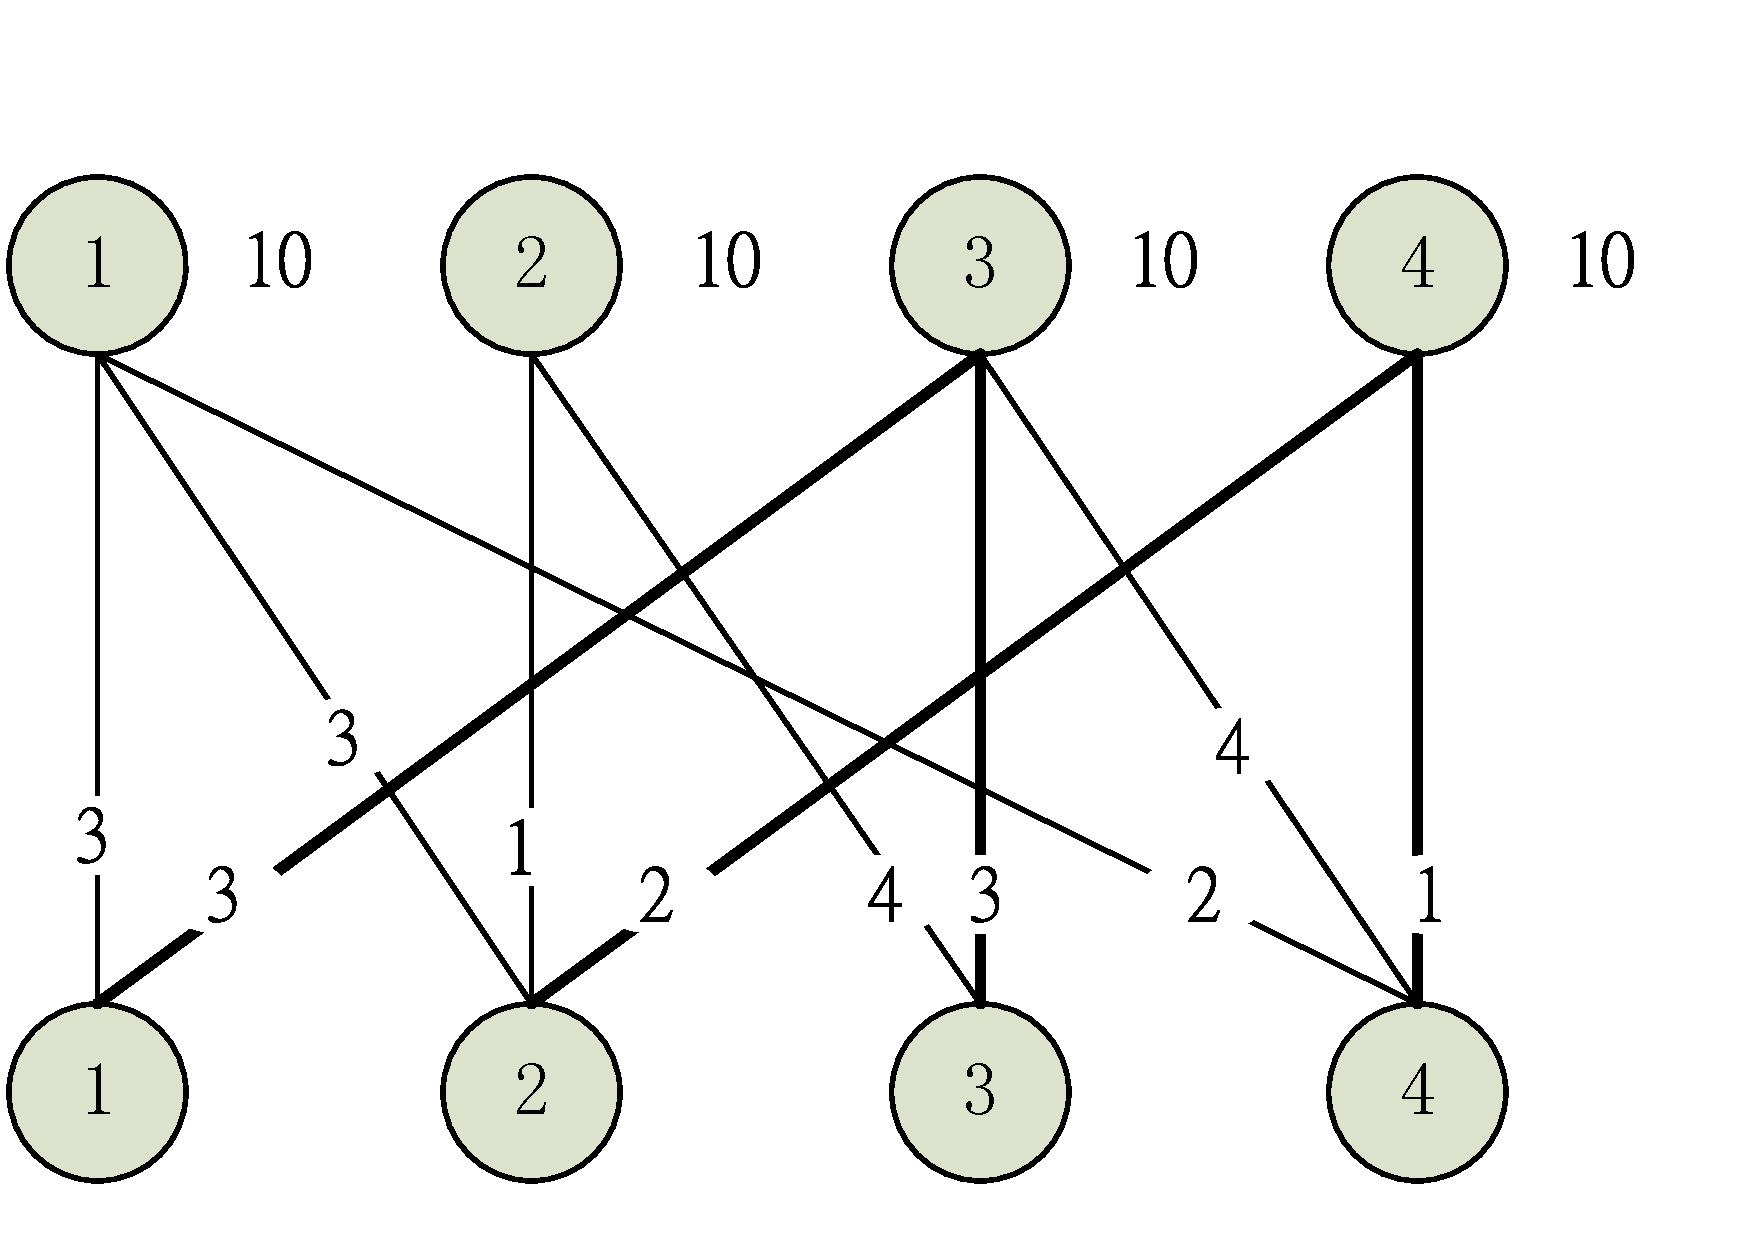
\includegraphics[width=0.5\textwidth]{preliminary-example.pdf}
\caption{\label{figure:exampleUFL}An example of a UFL game}
\vspace{-3mm}
\end{figure}

In the UFL game shown in Figure \ref{figure:exampleUFL}, there are four facilities and four customers (players). Each facility has a fixed opening cost 10. The numbers on the links are the transportation costs from facilities to customers. An optimal decision for the grand coalition is to open facilities 3 and 4, and the links in bold are the optimal paths. Therefore, the grand coalition cost is 10+10+3+3+2+1=29.

For this example, we use two LP solvers, the ``Simplex" and ``Interior Point" methods, in MATLAB Release 2011a to compute the LPB allocations, respectively.
Table \ref{table:UFLCA} shows the cost assigned to each player under different approaches.

\begin{table}[H]
\vspace{-2mm}
\centering
\tabcolsep=4pt
\small
\renewcommand\arraystretch{1.5}
\caption{\label{table:UFLCA} Optimal stable UFL cost allocations under different approaches}
\vglue5pt
\begin{tabular}[!h]{c c c c c c c c c c c c c}
\hline
\multicolumn{1}{c}{Method} &\multicolumn{1}{c}{} &\multicolumn{1}{c}{Player 1} &\multicolumn{1}{c}{} &\multicolumn{1}{c}{Player 2} &\multicolumn{1}{c}{} &\multicolumn{1}{c}{Player 3} &\multicolumn{1}{c}{} &\multicolumn{1}{c}{Player 4}	&\multicolumn{1}{c}{} &\multicolumn{1}{c}{Total Shared Cost}\\
\hline
LPB with Simplex	& &5.00	& &6.50	& &8.50	& &6.50	&	&26.5	&\\
LPB with Interior Point	& &6.58	& &6.50	& &8.50	& &4.92	&	&26.5	&\\
LRB	& &6.87	& &6.50	& &8.50	& &4.63	&	&26.5	&\\
\hline
\end{tabular}
\vspace{-3mm}
\end{table}


The example reveals that the LRB algorithm can generate optimal stable cost allocations that are different from those generated by common LP solvers.
The LRB solution is beyond the range of convex combination of the two LPB solutions. 
This demonstrates the value of the LRB algorithm in providing alternative cost allocations.


To investigate the capability of the LRB algorithm under a general setting, we tested 30 uncapacitated facility location benchmark instances developed by \cite{Benchmark}, all with $m=n=100$. We conducted all computational experiments  on a Windows 7 PC with an Intel Core i7-2600 running at 3.4GHz and 16G RAM. All algorithms were implemented in MATLAB Release 2011a.
Among the 30 instances there are 22 for which the LRB solution is  beyond the range of convex combination of the two LPB solutions. 
Again, this shows the value of the LRB algorithm in terms of computationally finding alternative optimal stable cost allocations even in cases where the LPB cost allocations are shown to be optimal.


\subsection{The NLCFL Game}\label{section:NLCFL}
In a Non-Linear single source Capacitated Facility Location (NLCFL) game, there is a bipartite network $G=(M,N,E)$ defined similarly to the UFL game. Each potential facility site $i \in M$ now has a capacity $Q_i$, and each customer point $j \in N$ has a demand $q_j$. Every customer can only be served by a single facility.
In addition to the opening cost, each facility $i$ also has an operational cost that is increasing with the number of customers it is serving. To model the economy-of-scale effect, we use  a quadratic function  $\theta_i[h_i n_i - l_i\big(n_i \big)^2]$ to measure the operational cost, where $n_i$ is the number of customers served by facility $i$, and $\theta_i$, $h_i$ and $l_i$ are appropriate parameters ensuring the cost is concave and increasing  for $n_i \in [0,n]$. 


Unlike the UFL game in which players are only the customers in $N$, the player set of the NLCFL game includes both facility players in $M$ and customer players in $N$. Similar settings of the players can also be found in the bin packing games (e.g., see \citealt{Faigle1993,Liu2009}).
Our LRB algorithm can also handle the case where only customer players are involved. However, by including facility players, together with a non-linear cost function, we can demonstrate the broad range of applications to which our LRB algorithm can be applied.

%
%We need to point out that the definitions of game players for NLCFL and UFL are different. In UFL, players are the customers in $N$. However, in NLCFL, the player set includes both facility players $M$ and customer players $N$. Similar definitions can be found in other cases such as bin packing games (e.g., see \citealt{Faigle1993,Liu2009}).
%The new way of defining coalitions shows the broad range of applications that our LRB algorithm can be applied to.
%Our LRB algorithm can also handle the case where the NLCFL game contains only customer players.

%For the NLCFL game including only customer players, it is not subadditive as 
%The NLCFL game discussed here is subadditive while the case including only customers as players is not. Our LRB 
%
%Compared with the case where the NLCFL game only contains customer players, the game discussed here is subadditive
%
%We need to point out that the game definitions for NLCFL and UFL are different. In UFL, players are the customers in $N$. However, in NLCFL, the player set includes both facility players $M$ and customer players $N$. For an NLCFL game defined with only customers as players where any set of customers can choose any facilities to open,  a low-cost facility may be opened by different groups of customers. \hl{This leads to an impractical situation because the NLCFL problem assumes that each facility has a limited capacity.} \textcolor{blue}{In this case, although the demands of each coalition are within the capacity of the low-cost facility, the cumulative demands might violate the capacity constraint once the cooperation pattern is realized. This may cause impracticability of the NLCFL game.}
%\textcolor{red}{(The authors should argue more clearly why this is an "impractical" situation.)}
%\textcolor{blue}{Mathematically, the violation of capacity constraint} may make the grand coalition have a cost higher than a collection of small coalitions, i.e., not sub-additive. So it is necessary to include facility sites in the game player set in order to have a more properly defined game. Similar definitions can be found in other cases such as bin packing games (e.g., see \citealt{Faigle1993,Liu2009}).

 
We need the following additional notation in defining the NLCFL game:
\begin{table}[H]
\vspace{-2mm}
\centering
\tabcolsep=7pt
\small
\renewcommand\arraystretch{1.5}
\caption{\label{table:notations} New notation used in the NLCFL game}
\vglue5pt
\begin{tabular}[!h]{c c}
\hline
\multicolumn{1}{c}{Notation} &\multicolumn{1}{c}{Meaning}\\
\cline{1-2}
\multicolumn{1}{c}{$Q_i$} &\multicolumn{1}{l}{The capacity of facility $i$, $\forall i \in M$, $Q_i \in \Z^+$.}\\
\multicolumn{1}{c}{$q_j$} &\multicolumn{1}{l}{The demand of customer $j$, $\forall j \in N$, $q_j \in \Z^+$.}\\ 
\multicolumn{1}{c}{$s$} &\multicolumn{1}{l}{A player coalition, $s = s_f \cup s_c$.}\\
\multicolumn{1}{c}{$s_f$} &\multicolumn{1}{l}{Facility player set in coalition $s$, $s_f \subseteq M$.}\\
\multicolumn{1}{c}{$s_c$} &\multicolumn{1}{l}{Customer player set in coalition $s$, $s_c \subseteq N$.}\\
\multicolumn{1}{c}{$\gamma^s$} &\multicolumn{1}{l}{Incidence vector $\big[ \gamma^{s_f}_1,\gamma^{s_f}_2,...,\gamma^{s_f}_{m},\gamma^{s_c}_{1},\gamma^{s_c}_{2},...,\gamma^{s_c}_{n} \big]^T$, where $\gamma^{s_f}_i=1$, if $i \in s_f$ and $\gamma^{s_f}_i=0$, }\\
\multicolumn{1}{c}{} &\multicolumn{1}{l}{otherwise; $\gamma^{s_c}_j=1$ if $j \in s_c$ and $\gamma^{s_c}_j=0$ otherwise, $\forall j \in N, s_f \subseteq M, s_c \subseteq N$.}\\
\hline
\end{tabular}
\vspace{-3mm}
\end{table}


\begin{definition}
An NLCFL game $\big( M \cup N,c_{NLCFL} \big)$ is defined with players in $M \cup N$, where $M$ is the facility player set, $N$  is the customer player set, and the characteristic function $c_{NLCFL}(s)$ is determined by NLP
\begin{equation}\label{eqn:cfobjnonlinear}
c_{NLCFL}(s_f \cup s_c) = \min_{v,u}  \sum_{i \in M} f_iv_i + \sum_{i \in M}\sum_{j \in N} c_{ij}u_{ij} + \sum_{i \in M} \theta_i \big[ \sum_{j \in N}h_iu_{ij} - l_i \big(\sum_{j \in N}u_{ij}\big)^2 \big]
\end{equation}
\begin{equation}\label{eqn:concf1}
s.t.~\sum_{i \in M} u_{ij} \geq \gamma_j^{s_c},~\forall j \in N,
\end{equation}
\begin{equation}\label{eqn:concf2}
\sum_{j \in N}q_ju_{ij} - Q_iv_i \leq 0, ~\forall i \in M,
\end{equation}
\begin{equation}\label{eqn:concf4}
v_i \leq \gamma_i^{s_f},~\forall i \in M,
\end{equation}
\begin{equation}\label{eqn:concf7}
 v_i,u_{ij}, \in \big\{0,1\big\},~\forall i \in M, j \in N.
\end{equation}
\end{definition} 
Compared with $c_{UFL}(s)$, $c_{NLCFL}(s_f \cup s_c)$ has a few new constraints. 
Constraints $(\ref{eqn:concf2})$ represent the capacity restrictions of the facilities; constraints $(\ref{eqn:concf4})$ ensure that only if a facility player is in the coalition can the corresponding facility be used to serve customers.


Since the objective function of $c_{NLCFL}(s_f \cup s_c)$ has a non-linear term to measure the facility operational cost, the LPB algorithm is no longer applicable to computing cost allocations. Next we will illustrate the implementation of the LRB algorithm on the NLCFL game.


\subsubsection{LRB Cost Allocation for the NLCFL Game}\label{example-decompnlcfl}
In the NLCFL characteristic function $c_{NLCFL}(s_f \cup s_c)$, by adding a new set of constraints
\begin{equation}\label{eqn:CFLLRBR}
u_{ij} \leq \gamma_i^{s_f}, ~u_{ij} \leq \gamma_j^{s_c},~\forall i \in M, j \in N,
\end{equation}
and then bringing constraints $\big\{\sum_{i \in M} u_{ij} \geq \gamma_j^{s_c}:\forall j \in N\big\}$ into the objective function with non-negative Lagrangian multiplier $\sigma$, we can derive the NLCFL Lagrangian characteristic function,
\begin{eqnarray*}\label{eqn:LRCFnonlinear}
\begin{aligned}
\begin{split}
c_{LR\_NLCFL}(s;\sigma) = \sum_{i \in M}f_iv_i + &\sum_{i \in M} \sum_{j \in N} \big(c_{ij} - \sigma_{j} + \theta_ih_i\big)u_{ij}
 - \sum_{i \in M} \theta_il_i \big( \sum_{j \in N}u_{ij}\big)^2 + \sum_{j \in N} \sigma_j \gamma_j^{s_c}\\
s.t.~&\sum_{j \in N}u_{ij}q_j - Q_iv_i \leq 0,~\forall i \in M,\\
~~~~~~&~~u_{ij} \leq \gamma_i^{s_f},~\forall i \in M, j \in N,\\
~~~&~~~~~~v_i \leq \gamma_i^{s_f},~\forall i \in M,\\
~~~~~~&~~u_{ij} \leq \gamma_j^{s_c},~\forall i \in M, j \in N,\\
v_i&, u_{ij} \in \{0,1\}, ~\forall i \in M, j \in N.
\end{split}
\end{aligned}
\end{eqnarray*}
Similar to constraints $(\ref{eqn:UFLLRBC})$ for $c_{UFL}$, the augmentation of constraints $(\ref{eqn:CFLLRBR})$ is to strengthen the Lagrangian lower bound for $c_{NLCFL}(s_f \cup s_c)$.

%Note that constraints $(\ref{eqn:CFLLRBR})$ can help to obtain a sharper Lagrangian lower bound for $c_{NLCFL}(s_f \cup s_c)$, and consequently, a better LRB cost allocation.

Following the LRB algorithm, we can decompose $c_{LR\_NLCFL}(\ \cdot\ ;\sigma)$ into $c_{LR1\_NLCFL}(\ \cdot\ ;\sigma)$ and $c_{LR2\_NLCFL}(\ \cdot\ ;\sigma)$ such that $c_{LR\_NLCFL}(s_f \cup s_c;\sigma) = c_{LR1\_NLCFL}(s_f \cup s_c;\sigma) + c_{LR2\_NLCFL}(s_f \cup s_c;\sigma)$, for all $s_f \subseteq M$ and $s_c \subseteq N$, and define NLCFL sub-game 1 $\big(M \cup N;c_{LR1\_NLCFL}(\ \cdot\ ;\sigma)\big)$ and NLCFL sub-game 2 $\big(M \cup N;c_{LR2\_NLCFL}(\ \cdot\ ;\sigma)\big)$, respectively.

For NLCFL sub-game 1, the characteristic function is
\begin{eqnarray}\label{eqn:ncgcf}
\begin{aligned}
\begin{split}
c_{LR1\_NLCFL}(s_f \cup s_c,\sigma) = \sum_{j \in N} \sigma_j\gamma_j^{s_c}.
\end{split}
\end{aligned}
\end{eqnarray}
According to Lemma $\ref{lemma:lr1core}$, we can derive the core cost allocation for game $\big(M \cup N, c_{LR1\_NLCFL}(\ \cdot \ ;\sigma)\big)$, where each customer player $j \in N$ is assigned a cost exactly equal to the Lagrangian dual price of serving her, and no facility players are assigned any cost since they do not need to be served. The cost allocation is given by $\alpha_{LR1\_NLCFL}^{\sigma}(j) = \sigma_j$ for all $j \in N$, and $\alpha_{LR1\_NLCFL}^{\sigma}(i) = 0$ for all $i \in M$.


For NLCFL sub-game 2, the characteristic function is
\begin{eqnarray*}
\begin{aligned}
\begin{split}
c_{LR2\_NLCFL}(s_f \cup s_c;\sigma) = \min_{v,u}& \sum_{i \in M} f_iv_i + \sum_{i \in M}\sum_{j \in N} \big(c_{ij} - \sigma_j + \theta_ih_i\big) u_{ij} - \sum_{i \in M} \theta_il_i \Bigl( \sum_{j \in N}u_{ij}\Bigr)^2\\
s.t.~&\sum_{j \in N}u_{ij}q_j - Q_iv_i \leq 0,~\forall i \in M,\\
~~~~&~~u_{ij} \leq \gamma_i^{s_f},~\forall i \in M, j \in N,\\
&~~~~~~v_i \leq \gamma_i^{s_f},~\forall i \in M,\\
~~~~&~~u_{ij} \leq \gamma_j^{s_c},~\forall i \in M, j \in N,\\
v_i&, u_{ij} \in \{0,1\}, ~\forall i \in M, j \in N.
\end{split}
\end{aligned}
\end{eqnarray*}

To solve $c_{LR2\_NLCFL}(s_f \cup s_c;\sigma)$, we can decompose it by facilities, i.e., $c_{LR2\_NLCFL}(s_f \cup s_c;\sigma) = \sum_{i \in s_f} \psi^i(s_c;\sigma)$, where for each $i \in s_f$,
\begin{eqnarray}\label{eqn:psi}
\begin{aligned}
\begin{split}
\psi^i(s_c;\sigma) = \min_{v_i,u_{ij}} f_iv_i + \sum_{j \in s_c} \big(c_{ij} - \sigma_j + \theta_ih_i\big)& u_{ij} - \theta_il_i \Bigl( \sum_{j \in s_c}u_{ij}\Bigr)^2\\
s.t. ~~ \sum_{j \in s_c}q_ju_{ij} - Q_iv_i \leq 0,&\\
v_i,u_{ij} \in \big\{0,1\big\},~\forall j \in s_c&.
\end{split}
\end{aligned}
\end{eqnarray}


It can be seen that each problem $\psi^i(s_c;\sigma)$ corresponds to a variant of the knapsack problem with an objective of minimizing a non-linear total value function, where $Q_i$ is the knapsack capacity, and $s_c$ is a set of items with each item $j\in s_c$ having a weight $q_j$ and a value $(c_{ij}-\sigma_j+\theta_ih_i)$.
In addition to the total value of the items packed into the knapsack, one can obtain an extra value $-\theta_il_i \Bigl( \sum_{j \in s_c}u_{ij}\Bigr)^2$, which is quadratic in the number of the items packed. When all weights $q_j$ are integers, we can solve $\psi^i(s_c;\sigma)$ by a dynamic program in pseudo-polynomial time $O(Q_in^2)$. 
\colorbox{yellow}{To be specific,} we define $F^{s_c}_i(j,k,q)$ as the minimum value of $\sum_{j'\in s_c,j'\leq j}(c_{ij'}-\sigma_{j'}+\theta_ih_i)u_{ij'}$ such that $\sum_{j'\in s_c,j'\leq j}u_{ij'}=k$ and $\sum_{j'\in s_c,j'\leq j}q_{j'}u_{ij'}\leq q$. 
\colorbox{yellow}{In other words,} $F^{s_c}_i(j,k,q)$ represents the minimum item value packed by including exactly $k$ items from set $\{1,2,\cdots,j\}$ within capacity $q$.
The dynamic programming recursion is as follows:
\begin{eqnarray*}
\begin{aligned}
\begin{split}
F^{s_c}_i(j,k,q)=\left\{
\begin{array}{ll}
F^{s_c}_i(j,k,q), & \mbox{ if } j\not\in s_c,
\\[3mm]
\min\big\{F^{s_c}_i(j-1,k,q),F^{s_c}_i(j-1,k-1,q-q_j) \big\}, & \mbox{ if } j\in s_c, 
\end{array}\right.
\end{split}
\end{aligned}
\end{eqnarray*}
with initial conditions $F^{s_c}_i(0,0,q)=0$ for  $q\geq 0$, and boundary conditions $F^{s_c}_i(j,k,q)=+\infty$ for $q<0$. Then $\psi_i(s_c;\sigma)$ can be found by $\psi_i(s_c;\sigma) = \min_{k\leq |s_c|}\bigl\{ 0, f_i+F^{s_c}_i(n,k,Q_i)-\theta_i l_i k^2\bigr\}$, and we have $c_{LR2\_NLCFL}(s_f \cup s_c;\sigma) = \sum_{i \in s_f} \psi_i(s_c;\sigma)$.




%Let $\kappa^{i}(s_c;\sigma)$ be the optimal value of the knapsack problem. 
%Then we have $\psi^{i}(s_c;\sigma)=\min\big\{0,f_i - \kappa^{i}(s_c;\sigma)\big\}$ and $c_{LR2\_NLCFL}(s_f \cup s_c;\sigma) = \sum_{i \in s_f} \min\big\{0,f_i - \kappa^{i}(s_c;\sigma)\big\}$.

Now we are ready to compute the optimal stable cost allocation $\alpha_{LR2\_NLCFL}^{\sigma}$ for NLCFL sub-game 2 by  the CGB algorithm, where we need to solve a pricing problem. In this particular case, the pricing problem is to find a coalition (or column) $s=s_f \cup s_c$ with the smallest reduced cost, where the reduced  cost for each $s = s_f \cup s_c$ is given by
\begin{eqnarray}\label{eqn:pricing1nlcfl}
\begin{aligned}
\begin{split}
\min_{v,u}  \sum_{i \in s_f} f_i v_i + \sum_{i \in s_f}\sum_{j \in s_c} &\big(c_{ij} - \sigma_j + \theta_ih_i\big)u_{ij} - \sum_{i \in s_f} \theta_il_i \Bigl( \sum_{j \in s_c}u_{ij}\Bigr)^2 - \sum_{k \in M \cup N} \gamma^s_k \pi_k^*\\ 
&s.t. ~~\sum_{j \in s_c}q_ju_{ij} \leq Q_iv_i, ~\forall i \in s_f,\\
&v_i, u_{ij} \in \big\{0,1\big\},~\forall i \in s_f, j \in s_c,
\end{split}
\end{aligned}
\end{eqnarray}
with $\pi^*$ being the optimal dual of the corresponding master problem for NLCFL sub-game 2. 


For each given $s=s_f\cup s_c$, one can obtain the optimal objective value of $(\ref{eqn:pricing1nlcfl})$ directly, as it equals $\sum_{i\in s_f}\psi^{i}(s_c;\sigma)-\sum_{k \in M \cup N} \gamma^s_k \pi_k^*$, where each $\psi^{i}(s_c;\sigma)$, as shown earlier, can be computed by dynamic programming. However, due to the exponential number of coalitions, it is computationally intractable to find a column $s$ with the most negative reduced cost by enumeration. We therefore attempt to first identify a column $\bar{s}$ with a negative reduced cost by considering the following two cases:
%, which is sufficient to ensure the correctness of the CGB algorithm. Consider two cases as follows:
%by enumeration. In addition, before the CGB algorithm is completed, it is actually not necessary to find the optimal column $s^*$ with the most negative reduced cost; any column $\bar{s}$ with a negative reduced cost can be used. To this end, we slightly shift our efforts to find such an $\bar s$, where we consider two cases.

Case 1: There exists at least one $k$ such that $\pi^*_k>0$. In this case, a coalition $\bar s$ can be defined by including $k$ with $\pi^*_k>0$ for $k\in M \cup N$. The reduced cost for $\bar s$ is negative because it is at most $-\sum_{k\in M\cup N} \max\{0, \pi^*_k\}$ by setting all $u$ and $v$ to be zero.

\colorbox{yellow}{Case 2: For all} $k\in M\cup N$,  $\pi^*_k \leq 0$. This case is more complicated. 
To efficiently find a coalition $\bar s = \bar{s}_f \cup \bar{s}_c$ with  a negative reduced cost, we can consider the following ILP where binary variables $v_i$ and $\gamma_j$ indicate 
whether or not $\bar{s}$ includes facility players $i$ and customer player $j$ with $f'_i = f_i - \pi_i^*$, $c'_{ij} = c_{ij}-\sigma_j + \theta_ih_i$, $l'_i = \theta_il_i$ and $\pi'_j = -\pi_j^*$. 
\begin{eqnarray}\label{eqn:pricing2nonlinear}
\begin{aligned}
\begin{split}
\min_{v;u;\gamma} R(v,u,\gamma) = \min_{v,u} &\sum_{i \in M} f'_i v_i + \sum_{i \in M}\sum_{j \in N} c'_{ij}u_{ij} - \sum_{i \in M} l'_i \big(\sum_{j \in N}u_{ij}\big)^2+ \sum_{j \in N} \gamma_j \pi'_j\\ 
s.t.&~~\sum_{j \in N}q_ju_{ij} \leq Q_iv_i, ~\forall i \in M,\\
&u_{ij} \leq \gamma_j,~\forall i \in M, j \in N,\\
v_i, u_{ij}&, \gamma_j \in \big\{0,1\big\},~\forall i \in M, j \in N,
\end{split}
\end{aligned}
\end{eqnarray}
\colorbox{yellow}{Therefore, it} can be seen that feasible solutions to ILP of negative objective values are one-to-one correspondence with coalitions $\bar{s} =  ̄\bar{s}_f \cup \bar{s}_c$ of negative reduced costs. Moreover, such a coalition $\bar{s}$ can be obtained efficiently by exploiting the properties below:

\begin{lemma}\label{lemma:efficientconditions}
For $(\ref{eqn:pricing2nonlinear})$, without changing the optimal objective value, one can sequentially fix some variables to zero by the following steps:\\
{\rm (1)} For each $(i,j)\in M\times N$, if $c'_{ij} - l'_i\big[n_i^2 - (n_i-1)^2\big] > 0$, then $u_{ij}=0$, where $n_i$ is the number of elements in set $\{c'_{ij} < \infty: \forall j \in N\}$. After that, set $c'_{ij}=\infty$.\\
{\rm (2)} For each $j\in N$, if $\pi'_j+\sum_{i\in M}\min\{c'_{ij}- l'_i\big[n_i^2 - (n_i-1)^2\big],0\} \geq 0$, then $\gamma_j=0$, $ u_{ij}=0$,  $\forall i\in M$. \\
{\rm (3)} For each $i\in M$, solve a non-linear knapsack problem similar to $(\ref{eqn:psi})$, where $Q_i$ is the knapsack capacity, and $N$ is the item set, with each item $j\in N$ having a weight $q_j$ and a value $c'_{ij}$. Let $\omega^i$ be the optimal objective function value of this knapsack problem. If   $\omega^{i} + f'_{i} \geq 0$, then set $v_i=0$ and $u_{ij}=0$, for all $j\in N$.
\end{lemma}
{\scshape Proof.}
First, if there exists a pair of indices $(i,j)$ such that $u_{ij} = 1$ and $c'_{ij} - l'_i\big[n_i^2 - (n_i-1)^2\big] > 0$ in a feasible solution of ILP $(\ref{eqn:pricing2nonlinear})$, one can directly set $u_{ij} = 0$, and derive another feasible solution under which the objective function value is reduced by at least $c'_{ij} - l'_i\big[n_i^2 - (n_i-1)^2\big]$.

Second, if there exists a customer $j$ such that $\gamma_j = 1$ and $\pi'_j+\sum_{i\in M}\min\{c'_{ij}- l'_i\big[n_i^2 - (n_i-1)^2\big],0\} \geq 0$ in a feasible solution of ILP $(\ref{eqn:pricing2nonlinear})$, then setting $\gamma_j = 0$ and $u_{ij} = 0$ for all $i \in M$ results in another feasible solution where the objective function value is reduced by at least  $\pi'_j+\sum_{i\in M}\min\{c'_{ij}- l'_i\big[n_i^2 - (n_i-1)^2\big],0\}$.

Third, if there exists a facility $i$ such that $v_i = 1$ and $\omega^{i} + f'_{i} \geq 0$ in a feasible solution of ILP $(\ref{eqn:pricing2nonlinear})$, then the resulting solution by setting $v_i = 0$ and $u_{ij} = 0$ for all $j \in N$ is also feasible and the objective function value is reduced by at least $\omega^{i} + f'_{i}$.
\hfill\Halmos


Suffice it to say that making the above changes does not increase the value of $\min_{v;u;\gamma} R(v,u,\gamma)$.
Though not theoretically ensuring polynomial time complexity, the steps  in Lemma $\ref{lemma:efficientconditions}$ can indeed greatly reduce the problem size when solving $(\ref{eqn:pricing2nonlinear})$. %This is supported by our computational results in Section \ref{sec:nlcflcomputation}.

After deriving the optimal stable cost allocations $\alpha_{LR1\_NLCFL}^{\sigma}$ and $\alpha_{LR2\_NLCFL}^{\sigma}$ for NLCFL sub-games 1 and 2, respectively, we can compute a stable cost allocation $\alpha_{LR\_NLCFL}^{\sigma} = \alpha_{LR1\_NLCFL}^{\sigma} + \alpha_{LR2\_NLCFL}^{\sigma}$ for an NLCFL game according to Theorem $\ref{thm:lrcostallocationfeasible}$. Furthermore, by Theorem $\ref{thm:lagcostallocation1}$, the corresponding LRB cost allocation value $\sum_{k \in M\cup N}\alpha^{\sigma^*}_{LR\_NLCFL}(k)$ is equal to the Lagrangian relaxation lower bound $c_{LR\_NLCFL}(M \cup N;\sigma^*)$, if $\sigma^*$ is the optimal Lagrangian multiplier and $\big(M \cup N;c_{LR2\_NLCFL}(\ \cdot\ ;\sigma^*)\big)$ has a non-empty core.




\subsubsection{Computational Results for the NLCFL Game}\label{sec:nlcflcomputation}
To conduct the computational experiments, we use 20 single source facility location benchmark instances developed by \cite{Benchmark}. Each instance has a bipartite network $G=(M,N,E)$ with $m=n=100$ and $f_i=100$ for all $i \in M$.   
For each instance, there are three capacity levels  10, 20 and 30. 
In addition, we use $h_1 = h_2 = ... = h_m = n^2$, $l_1 = l_2= ... = l_m = 1$, and $\theta_1 = \theta_2 = ... = \theta_m=\theta$ to measure the operational cost, where $\theta$ indicates the relative weight of the operational cost.
When solving the Lagrangian dual problem by the subgradient method, we set the number of maximal iterations to be $2500$.
%\textcolor{blue}{i.e., we will choose the Lagrangian multiplier with the sharpest lower bound within 2500 iterations as the best solution for the Lagrangian dual problem.}


To show the effectiveness of the LRB cost allocation, ideally we need to compare the total shared cost against the grand coalition cost $c_{NLCFL}(M \cup N)$.
However, the grand coalition cost is only available in the benchmark data set for instances with $\theta=\textbf{0}$. 
Therefore, for a general comparison, we need to compromise by replacing the centralized optimum with a heuristic solution, called the Best Found Centralized Solution (BFCS), which is defined as the better of the following two feasible solutions.
The first feasible solution is simply the optimal solution to the original benchmark instances of the NLCFL problems with $\theta = \textbf{0}$, which is available in \cite{Bachrach2009Cost}.
The second feasible solution is derived from the optimal solution of $c_{LR2\_NLCFL}(M \cup N;\sigma)$.
Note that this optimal solution might be infeasible for the centralized problem $c_{NLCFL}(M \cup N)$, since some customers may not be served. 
If so, to derive a feasible solution out of the given infeasible solution, we can proceed as follows. 
For each unserved customer, we choose an opened facility with enough remaining capacity and the smallest transportation cost to serve this customer; if there is no such facility, we open a new feasible facility with the minimum transportation cost to serve this customer.

Table $\ref{table:LRBNSG}$ shows the performance and computational efficiency of the LRB cost allocation algorithm implemented on the 20 instances under situations where the facility capacities are identically equal to 10, 20 and 30, respectively. 
\begin{table}[H]
\vspace{-2mm}
\centering
\tabcolsep=6pt
\small
\renewcommand\arraystretch{1.4}
\caption{\label{table:LRBNSG}Performance of LRB cost allocation algorithm for the NLCFL game}
\vglue5pt
\begin{tabular}[!h]{c c c c c c c c c c c c c c}
\hline
\multirow{2}{*}{Capacity} &\multirow{2}{*}{$\theta$} &\multicolumn{1}{c}{} & \multicolumn{3}{c}{LRCA / BFCS (\%)} &\multicolumn{1}{c}{} & \multicolumn{3}{c}{LRCA / LRB(\%)}  &\multicolumn{1}{c}{} & \multicolumn{3}{c}{Total time(s)}\\
\cline{4-6}
\cline{8-10}
\cline{12-14}
& & & Average & Max &Min	& & Average & Max &Min & & Average & Max &Min\\
\hline
\multirow{5}{*}{$Q=10$}
&0  &  &98.79	&99.12	&98.33	&	&100	&100	&100	&	&--	&--	&--\\

&0.01  &  &99.64	&99.70	&99.55	&	&100	&100	&100	&	&5683	&6838	&4987\\

&0.1  &  &99.87	&99.89	&99.78	&	&100	&100	&100	&	&5690	&6834	&4980\\

&0.5  &  &99.90	&99.92	&99.87	&	&100	&100	&100	&	&5742	&6814	&5036\\

&1  &  &99.91	&99.95	&99.89	&	&100	&100	&100	&	&5822	&6983	&4764\\
\hline
\multirow{5}{*}{$Q=20$}
&0  &  &98.32	&99.30	&97.66	&	&100	&100	&99.95	&	&--	&--	&--\\

&0.01  &  &99.61	&99.76	&99.48	&	&100	&100	&100	&	&9925	&10478	&9485\\

&0.1  &  &99.83	&99.85	&99.82	&	&100	&100	&100	&	&9835	&10458	&9322\\

&0.5  &  &99.85	&99.88	&99.84	&	&100	&100	&99.99	&	&9825	&10487	&9315\\

&1  &  &99.89	&99.92	&99.87	&	&100	&100	&100	&	&9973	&11154	&9812\\
\hline
\multirow{5}{*}{$Q=30$}
&0  &  &95.25	&96.95	&93.93	&	&100	&100	&100	&	&--	&--	&--\\

&0.01  &  &99.02	&99.15	&98.82	&	&100	&100	&99.99	&	&11686	&12831	&10410\\

&0.1  &  &99.72	&99.77	&99.63	&	&99.99	&100	&99.95	&	&11755	&12816	&10421\\

&0.5  &  &99.81	&99.87	&99.78	&	&100	&100	&100	&	&11485	&13064	&10277\\

&1  &  &99.88	&99.92	&99.86	&	&100	&100	&100	&	&12621	&14371	&11955\\
\hline
\end{tabular}
\vspace{-3mm}
\end{table}



In the table, ``LRCA'' represents the best found LRB cost allocation value $\sum_{k \in M \cup N}\alpha_{LR\_NLCFL}^{\sigma}(k)$ under different $\sigma$, and ``LRB'' represents the best Lagrangian lower bound $c_{LR\_NLCFL}(M \cup N; \sigma^*)$ obtained using the subgradient method. For each capacity, we list the computational results under different values of $\theta$.
From column ``LRCA/BFCS'' it can be seen that for all the examined instances, our LRB cost allocation algorithm can produce stable cost allocations that share at least $93.93\%$ of BFCS. When  $\theta$ increases so that the facility operational cost gains more weight, our LRB cost allocations can share more than $99\%$ of BFCS. 
These findings demonstrate the high quality of the LRB cost allocations. 
%\textcolor{blue}{~Liu: Moreover, although NLCFL sub-game 2 is not submodular in general, column ``LRCA / LRB" suggests that almost every NLCFL sub-game 2 has a non-empty core.
%Thus, the resulting LRB cost allocation value is very likely to equal the corresponding Lagrangian lower bound.
%This indicates the superiority of the LRB algorithm over the LPB algorithm, even in cases where condition (2) of Theorem \ref{thm:lagcostallocation1} does not hold.}
\colorbox{yellow}{Moreover, although} NLCFL sub-game 2 is not submodular in general, column ``LRCA / LRB" suggests that almost every NLCFL sub-game 2 has a non-empty core.
This indicates that even in cases where condition (2) of Theorem \ref{thm:lagcostallocation1} does not hold, the LRB cost allocation still has a great chance to achieve the Lagrangian lower bound.
%Thus, the resulting LRB cost allocation value is very likely to equal the corresponding Lagrangian lower bound.
%In particular, when $\theta=0$, the resulting LRB cost allocation value is very likely to equal the corresponding Lagrangian lower bound, and thus surpass the LP lower bound as well as the LPB cost allocation value.
%This indicates that even in cases where condition (2) of Theorem \ref{thm:lagcostallocation1} does not hold, the LRB algorithm still has a great chance to beat the LPB algorithm in terms of total allocated cost.}
As for time efficiency, we can see that the computational time tends to increase with $Q$ and $\theta$. Among all instances, the longest computation time is around four hours.



For instances with $\theta=\textbf{0}$, where the NLCFL game has no nonlinear term in its characteristic function, we compare the LPB and LRB cost allocations, by showing in Table \ref{table:LRBLPBSG} the percentage ratios of the cost allocation values against the grand coalition costs given by the benchmarks. Here the LPB and LRB cost allocations are computed based on the same ILP formulation for the characteristic function $c_{NLCFL}(s_f \cup s_c)$ augmented by constraints $(\ref{eqn:CFLLRBR})$.


\begin{table}[H]
\vspace{-2mm}
\centering
\tabcolsep=14pt
\small
\renewcommand\arraystretch{1.5}
\caption{\label{table:LRBLPBSG}LPB vs. LRB cost allocations for the NLCFL game with $\theta = \textbf{0}$ (in \%)}
\vglue5pt
\begin{tabular}[!h]{c c c c c c c c c c}
\hline
\multirow{2}{*}{Capacity} & \multicolumn{5}{c}{Average}	&\multicolumn{1}{c}{} & \multicolumn{2}{c}{LRCA $-$ LPCA}\\
\cline{2-6}
\cline{8-9}
& LPCA & LRB & LRCA	& LRB$'$ & LRCA$'$	& &Max	&Min\\
\hline
10    &97.15	&98.79	&98.79	&98.79	&98.79	&	&2.38	&1.00\\

20    &97.20	&98.32	&98.31	&98.29	&98.25	&	&1.51	&0.88\\

30    &94.70	&95.25	&95.25	&95.21	&95.21	&	&0.75	&0.38\\

40    &94.11	&94.25	&94.25	&94.25	&94.25	&	&0.28	&0.07\\

50    &93.87	&93.88	&93.88	&93.88	&93.88	&	&0.04	&-0.02\\
\hline
\end{tabular}
\vspace{-3mm}
\end{table}
To study the impact of constraints $(\ref{eqn:CFLLRBR})$, we compare LRB and LRCA with a new Lagrangian lower bound LRB$'$ and a new LRB cost allocation value LRCA$'$, where LRB$'$ and LRCA$'$ are obtained from a revised characteristic function of $c_{LR_NLCFL}(s;\sigma)$ with constraints $(\ref{eqn:CFLLRBR})$ being relaxed. Moreover,
since the LPB cost allocation value and the LP lower bound are equal, they are both presented in column ``LPCA'' of Table~\ref{table:LRBLPBSG}.
%present in column ``LRB$'$" and column ``LRCA$'$" the optimal Lagrangian lower bounds and the best found LRB cost allocation values without augmenting $(\ref{eqn:CFLLRBR})$ to $c_{NLCFL}(s_f \cup s_c)$ , respectively.
From the table, we have the following observations:

First, the Lagrangian lower bound is tighter than the LP lower bound on average, as shown in the first two columns under ``Average''.
This implies the potential advantage of the LRB cost allocation over the LPB cost allocation.
In addition, as indicated by the columns under ``LRCA $-$ LPCA'', the LRB cost allocation is indeed superior to the LPB on average, especially for cases with a lower capacity.

%Second, indicated by column ``LRB $-$ LRCA'', the LRB cost allocation can achieve the Lagrangian lower bound in most cases, with only one exception at capacity 20 where the LRB cost allocation value is slightly different from the Lagrangian bound. Together with the columns under ``LRCA $-$ LPCA'', we can conclude that   the LRB cost allocation is indeed superior to the LPB on average, especially for cases with a lower  capacity.

Second, as shown in columns ``LRB, LRCA, LRB$'$, LRCA$'$", adding constraints $(\ref{eqn:CFLLRBR})$ to $c_{NLCFL}(s_f \cup s_c)$ can indeed improve the Lagrangian lower bounds, as well as the LRB cost allocation values. In addition, by comparing columns ``LPCA" and ``LRCA$'$", we find that even with no additional constraints, the resulting LRB cost allocation still beats the LPB one on average. This further implies the competitiveness of our LRB algorithm.



%For instances with $\theta=\textbf{0}$, where the NLCFL game has no nonlinear term in its characteristic function, we can compare the LPB and LRB cost allocations in Table 6. Here the LPB and LRB cost allocations are computed based on the same ILP formulation for the characteristic function that adds (26) to $c_{NLCFL}(s_f \cup s_c)$.

%Rows ``CFL" in Table \ref{table:LRBNSG} show the results for $\theta=\textbf{0}$, i.e., the case where the NLCFL game has no nonlinear term in its characteristic function. In the remaining section, we will present some more interesting computational results for this special case, denoted as the CFL game, as supplements to show the performances of the LRB algorithm.


We next investigate the convergence of the LRB algorithm on the NLCFL game. 
This was not an issue for the UFL game.
As long as the subgradient method for the Lagrangian dual problem converges to $\sigma^*$ in a UFL game, Theorem~\ref{thm:lagcostallocation1} ensures the optimality of the stable cost allocation corresponding to $\sigma^*$ because UFL sub-game 2 has a non-empty core. 
However, the NLCFL sub-game 2 may have an empty core, implying a possible gap between the Lagrangian lower bound and the total cost that can be allocated.
Although we may expect a general trend where a tighter Lagrangian lower bound leads to a better cost allocation, there is no guarantee of the strict increase of cost allocation value when the Lagrangian lower bound increases.

%We first investigate the convergence of the LRB algorithm on the CFL game. This was not an issue for the UFL game. 
%As long as the subgradient method for the Lagrangian dual problem converges to $\lambda^*$ in a UFL game, Theorem~\ref{thm:lagcostallocation1} ensures the optimality of the stable cost allocation corresponding to $\lambda^*$ because UFL sub-game 2 has an non-empty core. 
%However, the CFL sub-game 2 may have an empty core, implying a possible gap between the Lagrangian lower bound and the total cost that can be allocated. 
%\textcolor{blue}{In addition, we did not mention the convergence issue in NLCFL game since its LRB cost allocation is too good to leave enough space for the observation of such convergence.}
%Although we may expect a general trend where a tighter Lagrangian lower bound leads to a better cost allocation, there is no guarantee of the strict increase of cost allocation value when the Lagrangian lower bound increases.

%\textcolor{blue}
%{To examine this, we apply Algorithm~\ref{algolrb} to the NLCFL game on instances with $\theta=\textbf{0}$, and choose the set $\Lambda$ to include Lagrangian multipliers that are obtained by setting the number of maximal iterations to be 500, 800, 1000, 1500, 2000 and 2500 in the subgradient method.
%The corresponding LRB cost allocations obtained from these multipliers are compared in Table~\ref{table:CFLIterations}.}
%\begin{table}[H]
%\vspace{-2mm}
%\centering
%\tabcolsep=9pt
%\small
%\renewcommand\arraystretch{1.5}
%\caption{\label{table:CFLIterations}Comparisons of LRB cost allocations derived from Lagrangian multipliers at different iterations}
%\vglue5pt
%\begin{tabular}[!h]{c c c c}
%\hline
%\multirow{1}{*}{Iterations} & \multicolumn{1}{c}{\# of Improved} & \multicolumn{1}{c}{\# of Declined}	& \multicolumn{1}{c}{\# of Unchanged}\\
%\hline
%$\big\{800\big\}$ vs. $\big\{500\big\}$   &95	&4	&1\\
%
%$\big\{1000\big\}$ vs. $\big\{500, 800\big\}$     &51	&6	&43\\
%
%$\big\{1500\big\}$ vs. $\big\{500,800,1000\big\}$     &24	&6	&70\\
%
%$\big\{2000\big\}$ vs. $\big\{500,800,1000,1500\big\}$     &1	&6	&93\\
%
%$\big\{2500\big\}$ vs. $\big\{500,800,1000,1500,2000\big\}$     &0	&7	&93\\
%\hline
%\end{tabular}
%\vspace{-3mm}
%\end{table}


\colorbox{yellow}{ To examine this, we }apply Algorithm~\ref{algolrb} to the NLCFL game on instances with $\theta=\textbf{0}$, and compare LRB cost allocations that are obtained by using different $\Lambda$ sets of Lagrangian multipliers. Table~\ref{table:CFLIterations} reports the number of instances whose LRB cost allocations are improved, declined, and unchanged, respectively, when $\Lambda$ is changed from a baseline set $\Lambda_2$ to another set $\Lambda_1$.
Each $\sigma^{i}$ represents the best Lagrangian multiplier found within $i$ iterations of the subgradient method in Step~1 of Algorithm~\ref{algolrb}. The results show that it is possible that the cost allocation may become worse as the Lagrangian bound improves, though the chance of getting worse is very small in later iterations. For example, out of the one hundred instances, there are seven instances whose LRB cost allocations decline in quality when $\Lambda$ is chosen to be $\{\sigma^{2500}\}$ instead of $\{\sigma^{500},\sigma^{800},\sigma^{1000},\sigma^{1500},\sigma^{2000}\}$. This finding confirms the need for using multiple Lagrangian multipliers in Algorithm~\ref{algolrb}.

\begin{table}[H]
\vspace{-2mm}
\centering
\tabcolsep=9pt
\small
\renewcommand\arraystretch{1.5}
\caption{\label{table:CFLIterations}
Comparisons of LRB cost allocations derived from different $\Lambda$ sets of Lagrangian multipliers}
\vglue5pt
\begin{tabular}[!h]{c c c c c}
\hline
\multicolumn{2}{c}{Pairs of $\Lambda$ sets} &\multirow{2}{*}{\# of Improved}	&\multirow{2}{*}{\# of Declined}	&\multirow{2}{*}{\# of Unchanged}\\
\cline{1-2}
$\Lambda_1$ &$\Lambda_2$ (as baseline) &\\
\hline
$\big\{\sigma^{800}\big\}$  &$\big\{\sigma^{500}\big\}$   &95	&4	&1\\

$\big\{\sigma^{1000}\big\}$ &$\big\{\sigma^{500}, \sigma^{800}\big\}$     &51	&6	&43\\

$\big\{\sigma^{1500}\big\}$ &$\big\{\sigma^{500},\sigma^{800},\sigma^{1000}\big\}$     &24	&6	&70\\

$\big\{\sigma^{2000}\big\}$ &$\big\{\sigma^{500},\sigma^{800},\sigma^{1000},\sigma^{1500}\big\}$     &1	&6	&93\\

$\big\{\sigma^{2500}\big\}$ &$\big\{\sigma^{500},\sigma^{800},\sigma^{1000},\sigma^{1500},\sigma^{2000}\big\}$     &0	&7	&93\\
\hline
\end{tabular}
\vspace{-5mm}
\end{table}


%\begin{table}[H]
%\vspace{-2mm}
%\centering
%\tabcolsep=9pt
%\small
%\renewcommand\arraystretch{1.5}
%\caption{\label{table:CFLIterations}
%Comparisons of LRB cost allocations derived from different $\Lambda$ sets of Lagrangian multipliers}
%\vglue5pt
%\begin{tabular}[!h]{c c c c}
%\hline
%\multirow{1}{*}{Pairs of $\Lambda$ sets} & \multicolumn{1}{c}{\# of Improved} & \multicolumn{1}{c}{\# of Declined}	& \multicolumn{1}{c}{\# of Unchanged}\\
%\hline
%$\big\{\sigma^{800}\big\}$ vs. $\big\{\sigma^{500}\big\}$   &95	&4	&1\\
%
%$\big\{\sigma^{1000}\big\}$ vs. $\big\{\sigma^{500}, \sigma^{800}\big\}$     &51	&6	&43\\
%
%$\big\{\sigma^{1500}\big\}$ vs. $\big\{\sigma^{500},\sigma^{800},\sigma^{1000}\big\}$     &24	&6	&70\\
%
%$\big\{\sigma^{2000}\big\}$ vs. $\big\{\sigma^{500},\sigma^{800},\sigma^{1000},\sigma^{1500}\big\}$     &1	&6	&93\\
%
%$\big\{\sigma^{2500}\big\}$ vs. $\big\{\sigma^{500},\sigma^{800},\sigma^{1000},\sigma^{1500},\sigma^{2000}\big\}$     &0	&7	&93\\
%\hline
%\end{tabular}
%\vspace{-5mm}
%\end{table}






%Now we present the comparison of the CFL LPB and LRB cost allocations in Table $\ref{table:LRBLPBSG}$, where we show the percentage ratios of the best found cost allocation values against the centralized optimum, provided by the benchmark, of the grand coalition problem. 
%%The detailed of procedures of obtaining the CFL LPB cost allocations are shown in Appendix \ref{section:CFL}.
%
%
%
%\begin{table}[H]
%\vspace{-2mm}
%\centering
%\tabcolsep=8pt
%\small
%\renewcommand\arraystretch{1.5}
%\caption{\label{table:LRBLPBSG}LPB vs. LRB cost allocations for the CFL game over the centralized optimum (in \%)}
%\vglue5pt
%\begin{tabular}[!h]{c c c c c c c c c c c c c}
%\hline
%\multirow{2}{*}{Capacity} & \multicolumn{5}{c}{Average} &\multicolumn{1}{c}{} & \multicolumn{2}{c}{LRB $-$ LRCA}	&\multicolumn{1}{c}{} & \multicolumn{2}{c}{LRCA $-$ LPCA}\\
%\cline{2-6}
%\cline{8-9}
%\cline{11-12}
%& LPCA & LRB & LRCA	& LRB$'$ & LRCA$'$ & &Max	&Min	& &Max	&Min\\
%\hline
%10    &97.15	&98.79	&98.79	&98.79	&98.79	&	&0.00	&0.00	&	&2.38	&1.00\\
%
%20    &97.20	&98.32	&98.31	&98.29	&98.25	&	&0.05	&0.00	&	&1.51	&0.88\\
%
%30    &94.70	&95.25	&95.25	&95.21	&95.21	&	&0.00	&0.00	&	&0.75	&0.38\\
%
%40    &94.11	&94.25	&94.25	&94.25	&94.25	&	&0.00	&0.00	&	&0.28	&0.07\\
%
%50    &93.87	&93.88	&93.88	&93.88	&93.88	&	&0.00	&0.00	&	&0.04	&-0.02\\
%\hline
%\end{tabular}
%\vspace{-3mm}
%\end{table}
%In the table, ``LPCA'' represents the CFL LPB cost allocation value $\sum_{k \in M \cup N}\alpha_{LP\_CFL}(k)$ as well as the LP lower bound $c_{LP\_CFL}(M \cup N)$. 
%To show the effect of adding constraints $(\ref{eqn:CFLLRBR})$ to $c_{LR\_NLCFL}(s;\sigma)$, we focus on its special case, i.e., the CFL game.
%The new optimal Lagrangian lower bounds and best found LRB cost allocation values without augmenting $(\ref{eqn:CFLLRBR})$ to $c_{CFL}(s_f \cup s_c)$ are presented in columns ``LRB$'$" and ``LRCA$'$", respectively.
%
%
%From the table, we have the following observations. First, the Lagrangian lower bound is tighter than the LP lower bound on average, as indicated by the first two columns under ``Average''. This implies the potential advantage of the LRB cost allocation over the LPB cost allocation. In fact, when the capacity is low, the Lagrangian lower bound is consistently higher than the LP lower bound. Only  when the capacity is increased up to 50, there are a few occasions where the LP lower bound is tighter.
%
%Second, indicated by column ``LRB $-$ LRCA'', the LRB cost allocation can achieve the Lagrangian lower bound in most cases, with only one exception at capacity 20 where the LRB cost allocation value is slightly different from the Lagrangian bound. Together with the columns under ``LRCA $-$ LPCA'', we can conclude that   the LRB cost allocation is indeed superior to the LPB on average, especially for cases with a lower  capacity.
%
%Third, as shown in columns ``LRB, LRCA, LRB$'$, LRCA$'$ ", adding constraints $(\ref{eqn:CFLLRBR})$ to $c_{CFL}(s_f \cup s_c)$ can indeed improve the Lagrangian lower bounds as well as the LRB cost allocation values. In addition, by comparing columns ``LPCA" and ``LRCA$'$", we can find that even with no additional constraints, the resulting LRB cost allocation still beats the LPB one on average. This further implies the competitiveness of our LRB algorithm.

In summary, from the computational experiments  we can conclude that the LRB algorithm is both effective and efficient in solving the OCAP for the NLCFL game.




\section{Conclusion}\label{sec:conclude}

The focus of this paper is on cooperative games whose core may be empty. We propose a generic framework to calculate a good stable cost allocation that satisfies coalitional stability and recovers the grand coalition cost as much as possible. In the literature, such a problem is usually treated by linear programming relaxation and duality techniques. 
We take the different approach of investigating Lagrangian relaxation techniques. 
Besides the competitiveness of the Lagrangian bound over the linear programming bound, our algorithm is not restricted to solving problems with assignable constraints and linear objective functions.

We demonstrate our new algorithm on two different facility location games, each representing a typical type of cooperative game that may be encountered. The computational experiments show that our algorithm can produce near-optimal cost allocations for all these games, outperforming the existing linear programming based algorithm. In fact, we have also successfully implemented our algorithm on other typical games, such as TSP games, e.g., see \colorbox{yellow}{\cite{liulindongthesis}.}

\section*{Acknowledgement}
The authors appreciate the constructive and detailed comments by two anonymous reviewers. The work is partially supported by Hong Kong RGC GRF grant No. 618311.

\bibliographystyle{ijocv081}
\bibliography{ComputingGoodCAforORGames}

\newpage
%Lagrangian relaxation is a proven tool in optimization. Therefore it should also play an important role in games originating from optimization problems. Currently we are working along this direction to tackle other related problems in cooperative games, e.g., to calculate least core and strategy-proof allocations.

%=====================================================================================================================
%=====================================================================================================================
% Appendix here
% Options are (1) APPENDIX (with or without general title) or
%             (2) APPENDICES (if it has more than one unrelated sections)
% Outcomment the appropriate case if necessary
%
% \begin{APPENDIX}{<Title of the Appendix>}
% \end{APPENDIX}
%
%   or
%
% \begin{APPENDICES}
% \section{<Title of Section A>}
% \section{<Title of Section B>}
% etc
% \end{APPENDICES}


\begin{APPENDICES}
\section{Column and Row Generation Approaches for IM Games} \label{section:LPBalgorithm}
We summarize the column generation approach and the row generation approach (LPB algorithm) discussed by \cite{Caprara2010LPB} in this section.

For the column generation approach, consider the definition of OCAP by LP $(\ref{eqn:OCAP})$. Its dual problem is:
\begin{equation}\label{eqn:lpbrow1}
\min_{\beta} \big\{ \sum_{s \in S}c(s)\beta_s:\sum_{s \ni k}\beta_s = 1,\forall k \in V,\beta_s \geq 0, s \in S \big\}.
\end{equation}
Denote by $Q^{x\gamma}$ the overall set of feasible solutions of ILP (\ref{eqn:orgc1}), i.e.,
$$
Q^{x\gamma} = \bigl\{ x \in \big\{0,1\big\}^{ t \times 1},\gamma \in \big\{0,1\big\}^{v \times 1}:Ax \geq B\gamma+D,A'x \geq B'\gamma+D',\gamma = \gamma^s,\forall s \in S  \bigr\}.$$
Then LP (\ref{eqn:lpbrow1}) can be re-formulated, for the purpose of doing   column generation, by enumerating all values in $Q^{x\gamma}$. Specifically,
for each $(\bar{x},\bar{\gamma}) \in Q^{x\gamma}$, define variable $\beta_{\bar{x},\bar{\gamma}}$ with cost $C\bar{x}$. We will have a master LP
\begin{equation}\label{eqn:lpbrow2}
\min_{\beta} \big\{ \sum_{(\bar{x},\bar{\gamma}) \in Q^{x\gamma}} (C\bar{x})\beta_{(\bar{x},\bar{\gamma})}: \sum_{(\bar{x},\bar{\gamma}) \in Q^{x\gamma}} \bar{\gamma}_k \beta_{(\bar{x},\bar{\gamma})}=1,\forall k \in V, \beta_{\bar{x},\bar{\gamma}}\geq 0, (\bar{x},\bar{\gamma})\in Q^{x\gamma} \big\}.
\end{equation}
Though the formulation is straightforward, the above column generation is difficult to solve because the pricing problem amounts to optimizing over $Q^{x\gamma}$, which is usually NP-hard in the strong sense.


As to the row generation approach, it needs to identify a set of so-called assignable constraints, analogous to the cutting-plane method for solving IP where tight valid constraints are added to sharpen the LP bound. We let $P_I^x = conv \big\{ x \in \big\{0,1\big\}^{ t \times 1}:Ax \geq B\textbf{1}+D,A'x \geq B'\textbf{1}+D'  \big\}$ and $P_{I}^{x\gamma} = conv ~Q^{x\gamma}$, where function $conv\{\cdot\}$ represents the convex hull of a vector. Note that $P_I^x$ is the convex hull of the integer solutions to (\ref{eqn:orgc1}).


\begin{definition}
A valid inequality $ax \geq b$ for $P_I^x$ is said to be $assignable$ if there exists a valid inequality $ax \geq b'\gamma$ for $P_I^{x\gamma}$ such that $\sum_{k \in V}b'_k = b$.
\end{definition}
%In plain words, a valid inequality for $P_I^x$ is assignable if it corresponds to a homogeneous inequality which is valid for $P_I^{x\gamma}$.


\begin{theorem}\label{thm:LPBthm}
For an IM game $(V,c)$, if there exists an LP $\min_{x} \{Cx:Ex \geq F\gamma\}$ that gives a lower bound to ILP (\ref{eqn:orgc1}), where all constraints $Ex \geq F\gamma$ are assignable, then vector $\alpha_{LP}^{EF}$ given by
\begin{equation*}\label{eqn:LPBca}
\alpha_{LP}^{EF}(k) = \sum_{l=1}^{m_E} f_{lk}\mu_l^*,~\forall k \in V,
\end{equation*}
is a stable cost allocation for the IM game, where $\mu^*$ is the LP dual variable value for an optimal solution to $\min_{x} \{Cx:Ex \geq F\textbf{1}\}$, and $m_E$ is the number of rows of matrix $E$.
In addition, the total shared cost $\sum_{k \in V}\alpha_{LP}^{EF}(k) = \min_{x} \{Cx:Ex \geq F\textbf{1}\}$.
\end{theorem}

In fact, Theorem \ref{thm:LPBthm} stands true if $\mu^*$ is relaxed to be an optimal solution to the dual of $\min_{x} \{Cx:Ex \geq F\textbf{1}\}$. The proof is straightforward based on the results in Caprara and Letchford (2010). We will apply the extended results in our analysis.

Note that $c_{LP}^{EF}(V)=\min_{x} \{Cx:Ex \geq F\textbf{1}\}$ gives an LP lower bound of the grand coalition cost $c(V)$.
According to Theorem $\ref{thm:LPBthm}$, the quality of the LPB cost allocation $\alpha_{LP}^{EF}$ greatly depends on the tightness of constraints set $\{Ex \geq F\textbf{1}\}$, i.e., the tighter the constraints set is, the better the resulting  LPB cost allocation $\alpha_{LP}^{EF}$ is. In addition, if given a basic optimal solution of $\min_{x} \{Cx:Ex \geq F\textbf{1}\}$, then the resulting $\mu^*$ can be regarded as the shadow prices of constraints $Ex \geq F\textbf{1}$, and therefore this leads to some LPB cost allocations with strong business insights. Such examples can be seen in the UFL LPB cost allocations.

Four IM games are investigated in Caprara and Letchford (2010), namely, the Uncapacitated Facility Location game, the Rooted and Unrooted Travelling Salesman games and the Vehicle Routing game. For each game, they give a tight constraint set such that the total shared cost $c_{LP}^{EF}(V)$ is no smaller than $c_{LP}(V)$, the LP lower bound of $c(V)$ from the original ILP formulation.




%\section{The Supplemental Proofs}\label{section:proofs}
%\subsection{Proof of Lemma \ref{lemma:UFLSubmodular}}
%{\scshape Proof.}
%Denote $a$ and $b$ as two players in $N$. To show the submodularity, we need to prove that, for any coalition $s \in N\setminus \big\{a,b\big\}$,
%\begin{equation}\label{ll14}
%c_{LR2\_UFL}(s \cup \{a\}; \sigma) - c_{LR\_UFL2}(s;\sigma) \geq c_{LR2\_UFL}(s \cup \big\{a,b\big\};\sigma) - c_{LR2\_UFL}(s \cup \{b\};\sigma).
%\end{equation}
%For each $i\in M$, let $\Delta_i(s;\sigma) = \min \{0, f_i + \sum_{j \in s} \min \{0, c_{ij} - \sigma_j\} \}$. To show (\ref{ll14}), it is  sufficient to show
%\begin{equation}\label{eqn:submodularufl}
%\Delta_i(s;\sigma) + \Delta_i(s \cup \{a,b\};\sigma) \leq \Delta_i(s \cup \{a\};\sigma) + \Delta_i(s \cup \{b\};\sigma), ~\forall s \in N/\big\{a,b\big\}. \end{equation} 
%Let $\rho(x)=\min\{0,x\}$, and define $x_{\hat{s}}= f_i + \sum_{j \in \hat{s}} \min \{0, c_{ij} - \sigma_j\}$ for each $\hat{s}\in \{s,s\cup\{a\},s\cup\{b\},s\cup\{a,b\}\}$. 
%It can be seen that $x_s+x_{s\cup\{a,b\}} = x_{s\cup \{a\}}+x_{s\cup\{b\}}$, and $x_{s\cup\{a,b\}}\leq \min\{x_{s\cup \{a\}},x_{s\cup\{b\}}\}\leq  \max\{x_{s\cup \{a\}},x_{s\cup\{b\}}\} \leq x_{s}$. 
%Thus, since $\rho(x)$ is a concave function on $x$, we have
%\begin{eqnarray*}
%  \rho(x_s) + \rho(x_{s\cup \{a,b\}}) \leq \rho(x_{s\cup\{a\}}) + \rho(x_{s\cup \{b\}}),
%\end{eqnarray*}
%from which we can obtain (\ref{eqn:submodularufl}) directly, and completes the proof of Lemma~\ref{lemma:UFLSubmodular}.
%\hfill\Halmos





%\subsection{Proof of Theorem \ref{lemma:lpbequallrbufl}}
%{\scshape Proof.}
%For the UFL game, we first show that the LRB cost allocation is optimal. As stated earlier, the LRB cost allocation achieves the Lagrangian lower bound $c_{LR\_UFL}(N;\sigma^*)$, which is not less than the LP lower bound $c_{LP\_UFL}(N)$. It is known that the LP lower bound equals the maximum total shared cost for the UFL game \citep{Kolen1983FacilityLocationGame,Goemans2000FacilityLocationGames}. Thus, the LRB cost allocation must be an optimal UFL cost allocation, and $c_{LR\_UFL}(N;\sigma^*)=c_{LP\_UFL}(N)$.
%
%We next prove that both the LRB cost allocation set and the LPB cost allocation set consist of all the optimal UFL cost allocations. It is known that the LPB cost allocation set consists of all the optimal UFL cost allocations \citep{Goemans2000FacilityLocationGames}. This implies that each LRB cost allocation must belong to the LPB cost allocation set. Therefore, it remains to show that each LPB cost allocation belongs to the LRB cost allocation set.
%
%Consider each LPB cost allocation  $\alpha_{LP\_UFL}(j)=\mu^*_j$ for $j \in N$ where  $\mu^*$ together with some $\delta^*$ form an optimal solution to the following dual problem of $c_{LP\_UFL}(N)$:
%\begin{eqnarray*}
%\begin{aligned}
%\begin{split}\label{eqn:UFLLRdual1}
% \max_{\mu,\delta} \sum_{j \in N}&\mu_j\\
%s.t.~\sum_{j \in N}\delta_{ij} = f_i&, ~\forall i \in M,\\
%\mu_j - \delta_{ij} \leq c_{ij}, ~\forall i& \in M, j \in N,\\
% \mu_j \geq 0, \delta_{ij} \geq 0,~\forall &i \in M, j \in N.
%\end{split}
%\end{aligned}
%\end{eqnarray*}
%For each $i\in M$, it can be seen that $f_i = \sum_{j\in N}\delta^*_{ij}$, and that $\delta^*_{ij}\geq \max\{0,\mu^*_j-c_{ij}\}$ for $j \in N$, which implies that \textcolor{blue}{$f_i \geq \sum_{j\in N}\max\{0,\mu^*_j-c_{ij}\}=-\sum_{j\in N}\min\{0,c_{ij}-\mu^*_j\}$.} Thus, 
%\begin{eqnarray}
%  \min\{0,f_i + \sum_{j\in N}\min\{0,c_{ij}-\mu^*_j\}\} =0, \mbox{ for each $i\in M$.} \label{eqn:cost}
%\end{eqnarray}
%Since $c_{LR2\_UFL}(N;\sigma)=\sum_{i=1}^{m}\min\{0,f_i+\sum_{j\in N}\min\{0,c_{ij}-\sigma_{j}\}\}$ \textcolor{blue}{for any Lagrangian multiplier $\sigma$}, by (\ref{eqn:cost}) we have  $c_{LR2\_UFL}(N;\mu^*) = 0$.
%This, together with $c_{LR1\_UFL}(N;\mu^*)=\sum_{j\in N}\mu^*_j$, implies that $c_{LR\_UFL}(N;\mu^*) = \sum_{j\in N}\mu^*_j = c_{LP\_UFL}(N)=c_{LR\_UFL}(N;\sigma^*)$.
%Hence, $\mu^*$ is an optimal Lagrangian multiplier.
%The resulting LRB cost allocation is then given by $\alpha^{\mu^*}_{LR\_UFL}(j) = \mu^*_j + \alpha^{\mu^*}_{LR2\_UFL}(j)$ for $j \in N$. Note that  for each $s\in S$, since $c_{LR2\_UFL}(s;\mu^*)\leq 0$ and $c_{LR2\_UFL}(s;\mu^*)\geq c_{LR2\_UFL}(N;\mu^*)=0$, we have $c_{LR2\_UFL}(s;\mu^*)=0$, which \textcolor{blue}{leads to} $\alpha^{\mu^*}_{LR2\_UFL}(j) = 0$ for $j\in N$.
%Therefore, we obtain that $\alpha^{\mu^*}_{LR\_UFL} = \mu^*$, \textcolor{blue}{implying that} each LPB cost allocation $\mu^*$ belongs to the LRB cost allocation set. This completes the proof of  Theorem~\ref{lemma:lpbequallrbufl}.
%\hfill\Halmos




%\subsection{Proof of Lemma \ref{lemma:efficientconditions}}
%{\scshape Proof.}
%First, if there exists a pair of indices $(i,j)$ such that $u_{ij} = 1$ and $c'_{ij} - l'_i\big[n_i^2 - (n_i-1)^2\big] > 0$ in a feasible solution of ILP $(\ref{eqn:pricing2nonlinear})$, one can directly set $u_{ij} = 0$, and derive another feasible solution under which the objective function value is reduced by at least $c'_{ij} - l'_i\big[n_i^2 - (n_i-1)^2\big]$.
%
%Second, if there exists a customer $j$ such that $\gamma_j = 1$ and $\pi'_j+\sum_{i\in M}\min\{c'_{ij}- l'_i\big[n_i^2 - (n_i-1)^2\big],0\} \geq 0$ in a feasible solution of ILP $(\ref{eqn:pricing2nonlinear})$, then setting $\gamma_j = 0$ and $u_{ij} = 0$, for all $i \in M$, results in another feasible solution and the objective function value is reduced by at least  $\pi'_j+\sum_{i\in M}\min\{c'_{ij}- l'_i\big[n_i^2 - (n_i-1)^2\big],0\}$.
%
%Third, if there exists a facility $i$ such that $v_i = 1$ and $-\omega^{i} + f'_{i} \geq 0$ in a feasible solution of ILP $(\ref{eqn:pricing2nonlinear})$, then the resulting solution by setting $v_i = 0$ and $u_{ij} = 0$, for all $j \in N$, is also feasible and the objective function value is reduced by at least $-\omega^{i} + f'_{i}$.
%\hfill\Halmos


\end{APPENDICES}






%=====================================================================================================================
%=====================================================================================================================

% References here (outcomment the appropriate case)

% CASE 1: BiBTeX used to constantly update the references
%   (while the paper is being written).
%\bibliographystyle{ormsv080} % outcomment this and next line in Case 1
%\bibliography{<your bib file(s)>} % if more than one, comma separated

% CASE 2: BiBTeX used to generate mypaper.bbl (to be further fine tuned)
%\input{mypaper.bbl} % outcomment this line in Case 2

%If you don't use BiBTex, you can manually itemize references as shown below.


%\bibliographystyle{nonumber}


%\bibliographystyle{chicago}


% Acknowledgments here
%\ACKNOWLEDGMENT{%
% Enter the text of acknowledgments here
%}% Leave this (end of acknowledgment)


% Appendix here
% Options are (1) APPENDIX (with or without general title) or 
%             (2) APPENDICES (if it has more than one unrelated sections)
% Outcomment the appropriate case if necessary
%
% \begin{APPENDIX}{<Title of the Appendix>}
% \end{APPENDIX}
%
%   or 
%
% \begin{APPENDICES}
% \section{<Title of Section A>}
% \section{<Title of Section B>}
% etc
% \end{APPENDICES}


% References here (outcomment the appropriate case) 

% CASE 1: BiBTeX used to constantly update the references 
%   (while the paper is being written).
%\bibliographystyle{ijocv081} % outcomment this and next line in Case 1
%\bibliography{<your bib file(s)>} % if more than one, comma separated

% CASE 2: BiBTeX used to generate mypaper.bbl (to be further fine tuned)
%\input{mypaper.bbl} % outcomment this line in Case 2

\end{document}


